\pdfoutput=1

\documentclass[review]{siamart0216}


\usepackage{amsmath,amssymb,amsfonts}
\newtheorem*{remark}{Remark}
\theoremstyle{assumption}
\newtheorem{assumption}{Assumption}

\usepackage[titletoc,toc,title]{appendix}

\usepackage{array} 
\usepackage{listings}
\usepackage{mathtools}
\usepackage{pdfpages}
\usepackage[textsize=footnotesize,color=green]{todonotes}
\usepackage{bm}
\usepackage{bbm}

\usepackage{tikz}
\usepackage[normalem]{ulem}
\usepackage{hhline}

\usepackage{graphicx}
\usepackage{subfig}
\usepackage{color}

%% ====================================== graphics

\usepackage{pgfplots}
\usepackage{pgfplotstable}
\definecolor{markercolor}{RGB}{124.9, 255, 160.65}
\pgfplotsset{
compat=1.3,
width=10cm,
tick label style={font=\small},
label style={font=\small},
legend style={font=\small}
}

\usetikzlibrary{calc}
\usetikzlibrary{intersections} 

%%% START MACRO FOR ANNOTATION OF TRIANGLE WITH SLOPE %%%.
\newcommand{\logLogSlopeTriangle}[5]
{
    % #1. Relative offset in x direction.
    % #2. Width in x direction, so xA-xB.
    % #3. Relative offset in y direction.
    % #4. Slope d(y)/d(log10(x)).
    % #5. Plot options.

    \pgfplotsextra
    {
        \pgfkeysgetvalue{/pgfplots/xmin}{\xmin}
        \pgfkeysgetvalue{/pgfplots/xmax}{\xmax}
        \pgfkeysgetvalue{/pgfplots/ymin}{\ymin}
        \pgfkeysgetvalue{/pgfplots/ymax}{\ymax}

        % Calculate auxilliary quantities, in relative sense.
        \pgfmathsetmacro{\xArel}{#1}
        \pgfmathsetmacro{\yArel}{#3}
        \pgfmathsetmacro{\xBrel}{#1-#2}
        \pgfmathsetmacro{\yBrel}{\yArel}
        \pgfmathsetmacro{\xCrel}{\xArel}

        \pgfmathsetmacro{\lnxB}{\xmin*(1-(#1-#2))+\xmax*(#1-#2)} % in [xmin,xmax].
        \pgfmathsetmacro{\lnxA}{\xmin*(1-#1)+\xmax*#1} % in [xmin,xmax].
        \pgfmathsetmacro{\lnyA}{\ymin*(1-#3)+\ymax*#3} % in [ymin,ymax].
        \pgfmathsetmacro{\lnyC}{\lnyA+#4*(\lnxA-\lnxB)}
        \pgfmathsetmacro{\yCrel}{\lnyC-\ymin)/(\ymax-\ymin)} % THE IMPROVED EXPRESSION WITHOUT 'DIMENSION TOO LARGE' ERROR.

        % Define coordinates for \draw. MIND THE 'rel axis cs' as opposed to the 'axis cs'.
        \coordinate (A) at (rel axis cs:\xArel,\yArel);
        \coordinate (B) at (rel axis cs:\xBrel,\yBrel);
        \coordinate (C) at (rel axis cs:\xCrel,\yCrel);

        % Draw slope triangle.
        \draw[#5]   (A)-- node[pos=0.5,anchor=north] {}
                    (B)-- 
                    (C)-- node[pos=0.5,anchor=west] {\textcolor{black}{#4}}
                    cycle;
    }
}
%%% END MACRO FOR ANNOTATION OF TRIANGLE WITH SLOPE %%%.

\newcommand{\logLogSlopeTriangleNeg}[5]
{
    % #1. Relative offset in x direction.
    % #2. Width in x direction, so xA-xB.
    % #3. Relative offset in y direction.
    % #4. Slope d(y)/d(log10(x)).
    % #5. Plot options.

    \pgfplotsextra
    {
        \pgfkeysgetvalue{/pgfplots/xmin}{\xmin}
        \pgfkeysgetvalue{/pgfplots/xmax}{\xmax}
        \pgfkeysgetvalue{/pgfplots/ymin}{\ymin}
        \pgfkeysgetvalue{/pgfplots/ymax}{\ymax}

        % Calculate auxilliary quantities, in relative sense.
        \pgfmathsetmacro{\xArel}{#1}
        \pgfmathsetmacro{\yArel}{#3}
        \pgfmathsetmacro{\xBrel}{#1-#2}
        \pgfmathsetmacro{\yBrel}{\yArel}
        \pgfmathsetmacro{\xCrel}{\xArel}

        \pgfmathsetmacro{\lnxB}{\xmin*(1-(#1-#2))+\xmax*(#1-#2)} % in [xmin,xmax].
        \pgfmathsetmacro{\lnxA}{\xmin*(1-#1)+\xmax*#1} % in [xmin,xmax].
        \pgfmathsetmacro{\lnyA}{\ymin*(1-#3)+\ymax*#3} % in [ymin,ymax].
        \pgfmathsetmacro{\lnyC}{\lnyA+#4*(\lnxA-\lnxB)}
        \pgfmathsetmacro{\yCrel}{\lnyC-\ymin)/(\ymax-\ymin)} % THE IMPROVED EXPRESSION WITHOUT 'DIMENSION TOO LARGE' ERROR.

        % Define coordinates for \draw. MIND THE 'rel axis cs' as opposed to the 'axis cs'.
        \coordinate (A) at (rel axis cs:\xArel,\yArel);
        \coordinate (B) at (rel axis cs:\xBrel,\yBrel);
        \coordinate (C) at (rel axis cs:\xCrel,\yCrel);

        % Draw slope triangle.
        \draw[#5]   (A)-- node[pos=.5,anchor=south] {}
                    (B)-- 
                    (C)-- node[pos=0.5,anchor=west] {\textcolor{black}{#4}}
                    cycle;
    }
}
%%% END MACRO FOR ANNOTATION OF TRIANGLE WITH SLOPE %%%.

%%% START MACRO FOR ANNOTATION OF TRIANGLE WITH SLOPE %%%.
\newcommand{\logLogSlopeTriangleFlipNeg}[5]
{
    % #1. Relative offset in x direction.
    % #2. Width in x direction, so xA-xB.
    % #3. Relative offset in y direction.
    % #4. Slope d(y)/d(log10(x)).
    % #5. Plot options.

    \pgfplotsextra
    {
        \pgfkeysgetvalue{/pgfplots/xmin}{\xmin}
        \pgfkeysgetvalue{/pgfplots/xmax}{\xmax}
        \pgfkeysgetvalue{/pgfplots/ymin}{\ymin}
        \pgfkeysgetvalue{/pgfplots/ymax}{\ymax}

        % Calculate auxilliary quantities, in relative sense.
        %\pgfmathsetmacro{\xArel}{#1}
        %\pgfmathsetmacro{\yArel}{#3}
        \pgfmathsetmacro{\xBrel}{#1-#2}
        \pgfmathsetmacro{\yBrel}{#3}
        \pgfmathsetmacro{\xCrel}{#1}

        \pgfmathsetmacro{\lnxB}{\xmin*(1-(#1-#2))+\xmax*(#1-#2)} % in [xmin,xmax].
        \pgfmathsetmacro{\lnxA}{\xmin*(1-#1)+\xmax*#1} % in [xmin,xmax].
        \pgfmathsetmacro{\lnyA}{\ymin*(1-#3)+\ymax*#3} % in [ymin,ymax].
        \pgfmathsetmacro{\lnyC}{\lnyA+#4*(\lnxA-\lnxB)}
        \pgfmathsetmacro{\yCrel}{\lnyC-\ymin)/(\ymax-\ymin)} % THE IMPROVED EXPRESSION WITHOUT 'DIMENSION TOO LARGE' ERROR.

	\pgfmathsetmacro{\xArel}{\xBrel}
        \pgfmathsetmacro{\yArel}{\yCrel}

        % Define coordinates for \draw. MIND THE 'rel axis cs' as opposed to the 'axis cs'.
        \coordinate (A) at (rel axis cs:\xArel,\yArel);
        \coordinate (B) at (rel axis cs:\xBrel,\yBrel);
        \coordinate (C) at (rel axis cs:\xCrel,\yCrel);

        % Draw slope triangle.
        \draw[#5]   (A)-- node[pos=0.5,anchor=east] {\textcolor{black}{#4}}
                    (B)-- 
                    (C)-- node[pos=0.5,anchor=north] {1}
                    cycle;
    }
}
%%% END MACRO FOR ANNOTATION OF TRIANGLE WITH SLOPE %%%.


%%% START MACRO FOR ANNOTATION OF TRIANGLE WITH SLOPE %%%.
\newcommand{\logLogSlopeTriangleFlip}[5]
{
    % #1. Relative offset in x direction.
    % #2. Width in x direction, so xA-xB.
    % #3. Relative offset in y direction.
    % #4. Slope d(y)/d(log10(x)).
    % #5. Plot options.

    \pgfplotsextra
    {
        \pgfkeysgetvalue{/pgfplots/xmin}{\xmin}
        \pgfkeysgetvalue{/pgfplots/xmax}{\xmax}
        \pgfkeysgetvalue{/pgfplots/ymin}{\ymin}
        \pgfkeysgetvalue{/pgfplots/ymax}{\ymax}

        % Calculate auxilliary quantities, in relative sense.
        %\pgfmathsetmacro{\xArel}{#1}
        %\pgfmathsetmacro{\yArel}{#3}
        \pgfmathsetmacro{\xBrel}{#1-#2}
        \pgfmathsetmacro{\yBrel}{#3}
        \pgfmathsetmacro{\xCrel}{#1}

        \pgfmathsetmacro{\lnxB}{\xmin*(1-(#1-#2))+\xmax*(#1-#2)} % in [xmin,xmax].
        \pgfmathsetmacro{\lnxA}{\xmin*(1-#1)+\xmax*#1} % in [xmin,xmax].
        \pgfmathsetmacro{\lnyA}{\ymin*(1-#3)+\ymax*#3} % in [ymin,ymax].
        \pgfmathsetmacro{\lnyC}{\lnyA+#4*(\lnxA-\lnxB)}
        \pgfmathsetmacro{\yCrel}{\lnyC-\ymin)/(\ymax-\ymin)} % THE IMPROVED EXPRESSION WITHOUT 'DIMENSION TOO LARGE' ERROR.

	\pgfmathsetmacro{\xArel}{\xBrel}
        \pgfmathsetmacro{\yArel}{\yCrel}

        % Define coordinates for \draw. MIND THE 'rel axis cs' as opposed to the 'axis cs'.
        \coordinate (A) at (rel axis cs:\xArel,\yArel);
        \coordinate (B) at (rel axis cs:\xBrel,\yBrel);
        \coordinate (C) at (rel axis cs:\xCrel,\yCrel);

        % Draw slope triangle.
        \draw[#5]   (A)-- node[pos=0.5,anchor=east] {\textcolor{black}{#4}}
                    (B)-- 
                    (C)-- node[pos=0.5,anchor=south] {}
                    cycle;
    }
}
%%% END MACRO FOR ANNOTATION OF TRIANGLE WITH SLOPE %%%.



\usepackage{stmaryrd}

\renewcommand{\hat}[1]{\hat{#1}}
\renewcommand{\topfraction}{0.85}
\renewcommand{\textfraction}{0.1}
\renewcommand{\floatpagefraction}{0.75}

\newcommand{\vect}[1]{\ensuremath\boldsymbol{#1}}
\newcommand{\tensor}[1]{\underline{\bm{#1}}}
\newcommand{\del}{\triangle}
\newcommand{\curl}{\grad \times}
\renewcommand{\div}{\grad \cdot}

\newcommand{\bbm}[1]{\mathbbm{#1}}
\newcommand{\bs}[1]{\boldsymbol{#1}}
\newcommand{\equaldef}{\stackrel{\mathrm{def}}{=}}

\newcommand{\td}[2]{\frac{{\rm d}#1}{{\rm d}{\rm #2}}}
\newcommand{\pd}[2]{\frac{\partial#1}{\partial#2}}
\newcommand{\nor}[1]{\left\| #1 \right\|}
\newcommand{\LRp}[1]{\left( #1 \right)}
\newcommand{\LRs}[1]{\left[ #1 \right]}
\newcommand{\LRa}[1]{\left\langle #1 \right\rangle}
\newcommand{\LRb}[1]{\left| #1 \right|}
\newcommand{\LRc}[1]{\left\{ #1 \right\}}
\newcommand{\LRceil}[1]{\left\lceil #1 \right\rceil}
\newcommand{\LRl}[1]{\left. #1 \right|}
\newcommand{\pdd}[2]{\frac{\partial^2#1}{\partial#2^2}}
\newcommand{\pdn}[3]{\frac{\partial^{#3}#1}{\partial#2^{#3}}}
\newcommand{\mb}[1]{\mathbf{#1}}
\newcommand{\mbb}[1]{\mathbb{#1}}
\newcommand{\mc}[1]{\mathcal{#1}}
\newcommand{\snor}[1]{\left| #1 \right|}


%\newcommand{\cond}[1]{\kappa\LRp{#1}}
\newcommand{\cond}[2]{\nor{#1}_{#2}\nor{{#1}^{-1}}_{#2}}


\newcommand{\Grad} {\ensuremath{\nabla}}
\newcommand{\Div} {\ensuremath{\nabla\cdot}}
\newcommand{\jump}[1] {\ensuremath{\llbracket#1\rrbracket}}
\newcommand{\avg}[1] {\ensuremath{\LRc{\!\{#1\}\!}}}

\newcommand{\Oh}{{\Omega_h}}
\renewcommand{\L}{L^2\LRp{\Omega}}
\newcommand{\LK}{L^2\LRp{D^k}}
\newcommand{\LdK}{L^2\LRp{\partial D^k}}
\newcommand{\Dhat}{\hat{D}}
\newcommand{\Lhat}{L^2\LRp{\Dhat}}

\renewcommand{\hat}{\widehat}

\newcommand{\eval}[2][\right]{\relax
  \ifx#1\right\relax \left.\fi#2#1\rvert}

\def\etal{{\it et al.~}}


\newcommand{\note}[1]{{\color{blue}{#1}}}
%\newcommand{\noteOne}[1]{{\color{blue}{#1}}}
%\newcommand{\noteTwo}[1]{{\color{red}{#1}}}
%\newcommand{\note}[1]{#1}
%\newcommand{\noteOne}[1]{#1}
%\newcommand{\noteTwo}[1]{#1}


\newcommand{\LinfDk}{L^{\infty}\LRp{D^k}}

\newcommand{\diag}[1]{{\rm diag}\LRp{#1}}

\newcommand{\Ksub}{K_{\rm sub}}

\newcolumntype{C}[1]{>{\centering\let\newline\\\arraybackslash\hspace{0pt}}m{#1}}

%% d in integrand
\newcommand*\diff[1]{\mathop{}\!{\mathrm{d}#1}}

\makeatletter
\renewcommand\d[1]{\mspace{6mu}\mathrm{d}#1\@ifnextchar\d{\mspace{-3mu}}{}}
\makeatother

\date{}
\author{Jesse Chan}%, David C.\ Del Rey Fernandez}
\title{Skew-symmetric entropy stable discontinuous Galerkin formulations}

\graphicspath{{./figs/}}

\begin{document}

\maketitle


\begin{abstract}
Entropy stable high order methods for nonlinear conservation laws satisfy an inherent discrete entropy inequality.  The construction of such schemes has relied on the use of carefully chosen collocation points \cite{gassner2013skew, fisher2013high, carpenter2014entropy, chan2018efficient} or volume and surface quadrature rules \cite{chan2017discretely, chan2018discretely} to produce operators which satisfy a summation-by-parts (SBP) property.  In this work, we show how to construct skew-symmetric schemes which are entropy stable even for volume and surface quadratures under which an SBP property does not hold.  These skew-symmetric formulations avoid the use of a ``strong'' SBP property, and require only that operators exactly differentiate constants and satisfy a discrete form of the fundamental theorem of calculus.  We conclude by discussing the applicability of these new operators for entropy stable schemes on hybrid meshes.% and non-conforming meshes.  
\end{abstract}

\section{Introduction}

High order methods for the simulation of time-dependent compressible flow have the potential to achieve higher levels of accuracy at lower costs compared to current low order schemes \cite{wang2013high}.  In addition to superior accuracy and efficiency on modern computing architectures, the low numerical dispersion and dissipation of high order methods \cite{ainsworth2004dispersive} enables the accurate propagation of waves over long distances and time scales.  The same properties also make high order methods attractive for the resolution of unsteady phenomena such as vorticular and turbulent flows, which are sensitive to numerical dissipation \cite{visbal1999high, wang2013high}.  However, while high order methods are often provably stable for wave problems, high order schemes for nonlinear conservation laws have consistently been hampered by problems of instability.  

When applied to nonlinear conservation laws, high order methods can experience artificial growth and blow-up near under-resolved features such as shocks, turbulence, or boundary layers.  In practice, the application of high order methods to practical problems requires shock capturing and stabilization techniques (such as artificial viscosity) or solution regularization (such as filtering or limiting) to prevent solution blow-up.  The resulting schemes for nonlinear conservation laws walk a fine line between stability, robustness, and accuracy.  Aggressive stabilization or regularization can result in the loss of high order accuracy, while too little can result in instability \cite{wang2013high}.  Moreover, it can be difficult to determine robust expressions for stabilization paramaters, as parameters which work for one simulation can fail when applied to a different physical regime or discretization setting.  

These issues have motivated the introduction of high order \textit{entropy stable} discretizations, which satisfy a semi-discrete entropy inequality while maintaining high order accuracy in smooth regions.  Proofs of continuous entropy inequalities rely on the chain rule.  In contrast, these discrete entropy inequalities account for the loss of the chain rule due to effects such as quadrature errors, which are incurred when applying polynomially exact quadrature rules to nonlinear and rational integrands within the DG formulation.  These schemes were first introduced as high order collocation methods on tensor product elements in \cite{fisher2013high, carpenter2014entropy, gassner2016split, gassner2017br1}, and were extended to simplicial elements in \cite{crean2017high, chen2017entropy, crean2018entropy, chan2017discretely, chan2018discretely}.  These methods have also been extended to staggered grid \cite{parsani2016entropy}, generalized SBP and Gauss nodes \cite{chan2018efficient} and non-conforming meshes \cite{friedrich2017entropy}.  Entropy stable boundary conditions have also been determined for the compressible Euler and Navier-Stokes equations \cite{parsani2015entropy, svard2018entropy}.  

\note{Finish: add Section description.  Talk about situations where the SBP or decoupled SBP property doesn't hold: triangles with reduced surface quadrature, GLL quads with GQ face quadratures, and hybrid couplings.}

\section{Entropy stability for systems of nonlinear conservation laws}

We begin by reviewing the dissipation of entropy for a $d$-dimensional system of nonlinear conservation laws on a domain $\Omega$
\begin{equation}
\pd{\bm{u}_h}{t}  + \sum_{j=1}^d\pd{\bm{f}_j(\bm{u})}{x_j} = 0, \qquad \bm{u}\in \mathbb{R}^n, \qquad \bm{f}:\mathbb{R}^n\rightarrow\mathbb{R}^n,
\label{eq:nonlineqs}
\end{equation}
where $\bm{u}$ are the conservative variables and $\bm{f}(\bm{u})$ is a vector-valued nonlinear flux function.  We are interested in nonlinear conservation laws for which a convex entropy function $U(\bm{u})$ exists.  For such systems, the  \emph{entropy variables} are an invertible mapping $\bm{v}(\bm{u}):\mathbb{R}^n\rightarrow \mathbb{R}^n$ defined as the derivative of the entropy function with respect to the conservative variables 
\begin{align}
\bm{v}(\bm{u}) = \pd{U}{\bm{u}}.%, \qquad  \text{ invertible}.%\bm{u}\LRp{\bm{v}(\bm{u})} = \bm{u}.
\label{eq:entropyvarsmap}
\end{align}
Several widely used equations in fluid modeling (Burgers, shallow water, compressible Euler and Navier-Stokes equations) yield convex entropy functions $U(\bm{u})$ \cite{hughes1986new, chen2017entropy}.  Let $\partial \Omega$ be the boundary of $\Omega$ with outward unit normal $\bm{n}$.  By multiplying the equation (\ref{eq:nonlineqs}) with $\bm{v}(\bm{u})^T$, the solutions $\bm{u}$ of (\ref{eq:nonlineqs}) can be shown to satisfy an entropy inequality
\begin{equation}
\int_{\Omega}\pd{U(\bm{u})}{t}\diff{x} + \int_{\partial \Omega} \sum_{j=1}^d \LRp{\bm{v}(\bm{u})^T\bm{f}_j(\bm{u}) - \psi_j\LRp{\bm{v}(\bm{u})}}n_j \diff{x} \leq 0, 
\label{eq:entropyineq}
\end{equation}
where $\bm{n} = \LRp{n_1,\ldots,n_d}$ denotes the outward unit normal, and $\psi_j(\bm{u})$ is some function referred to as the entropy potential.  

The proof of (\ref{eq:entropyineq}) requires the use of the chain rule \cite{mock1980systems, harten1983symmetric, dafermos2005compensated}.  The instability-in-practice of high order schemes for (\ref{eq:nonlineqs}) can be attributed in part to the fact that the discrete form of the equations do not satisfy the chain rule, and thus do not satisfy (\ref{eq:entropyineq}).  As a result, discretizations of (\ref{eq:nonlineqs}) do not typically possess an underlying statement of stability.  For low order schemes, this can be offset in practice by the inherent numerical dissipation.  However, because high order discretizations possess low numerical dissipation, the lack of an underlying discrete stability has been conflated with the idea that high order methods are inherently less stable than low order methods.

\section{Polynomial approximation spaces}

In this work, we consider either simplicial reference elements (triangles and tetrahedra) or tensor product reference elements (quadrilaterals and hexahedra).  We define an approximation space using degree $N$ polynomials on the reference element; however, the natural polynomial approximation space differs depending on the element type \cite{chan2015gpu}.  

On a $d$-dimensional reference simplex, the natural polynomial space are total degree $N$ polynomials 
\[
P^N\LRp{\hat{D}} = \LRc{\hat{x}_1^{i_1}\ldots\hat{x}_d^{i_d}, \quad \hat{\bm{x}} \in \hat{D}, \quad 0\leq \sum_{k=1}^d i_k \leq N}.
\]
In contrast, the natural polynomial space on a $d$-dimensional tensor product element is the space of maximum degree $N$ polynomials
\[
Q^N\LRp{\hat{D}} = \LRc{\hat{x}_1^{i_1}\ldots\hat{x}_d^{i_d}, \quad \hat{\bm{x}} \in \hat{D}, \quad 0\leq i_k \leq N, \quad k = 1,\ldots, d}.
\]
We denote the natural approximation space on a given reference element $\hat{D}$ by $V^N$.  Furthermore, we denote the dimension of $V^N$ as $N_p = {\rm dim}\LRp{V^N\LRp{\hat{D}}}$.  

The proofs presented in this work will also use anisotropic tensor product polynomial spaces, where the maximum polynomial degree varies depending on the coordinate direction.  We denote such spaces by $Q^{N_1, \ldots, N_d}$, where $N_k$ are non-negative integers and
\[
Q^{N_1, N_2, \ldots, N_d}\LRp{\hat{D}} = \LRc{\hat{x}_1^{i_1}\ldots\hat{x}_d^{i_d}, \quad \hat{\bm{x}} \in \hat{D}, \quad 0\leq i_k \leq N_k, \quad k = 1,\ldots, d}.
\]
For example, the isotropic tensor product space $Q^N$ is the same as $Q^{N,\ldots,N}$.

We also define trace spaces for each reference element.  Let $\hat{f}$ be a face of the reference element $\hat{D}$.  The trace space $V^N \LRp{\hat{f}}$ is defined as the restrictions of functions in $V^N\LRp{\hat{D}}$ to $\hat{f}$, and denote the dimension of the trace space as ${\rm dim}\LRp{V^N\LRp{{\hat{f}}}} = N^f_p$.  
\[
V^N \LRp{\hat{f}} = \LRc{ \left.u\right|_{\hat{f}}, \quad u \in V^N\LRp{\hat{D}}, \quad \hat{f}\in \partial\hat{D}}.
\]
For example, on a $d$-dimensional simplex, $V^N \LRp{\partial \hat{D}}$ consists of total degree $N$ polynomials on simplices of dimension $(d-1)$.  On a $d$-dimensional tensor product element, $V^N \LRp{\partial \hat{D}}$ consists of maximum degree $N$ polynomials on a tensor product element of dimension $(d-1)$.  

%For example, the trace space for degree $N$ polynomials on a quadrilateral face $\hat{f}$ of the bi-unit hexahedral element $[-1,1]^3$ is $Q^N\LRp{\hat{f}}$, while the trace space for degree $N$ polynomials on a triangular face $f$ of the tetrahedron is $P^N\LRp{\hat{f}}$.  


%We similarly define the trace space for the surface $\partial \hat{D}$ of $\hat{D}$
%\[
%V^N \LRp{\partial \hat{D}} = \LRc{ \left.u\right|_{\partial \hat{D}}, \quad u \in V^N\LRp{\hat{D}}}.
%\]
%For example, on a $d$-dimensional simplex, $V^N \LRp{\partial \hat{D}}$ consists of total degree $N$ polynomials on simplices of dimension $(d-1)$.  On a $d$-dimensional tensor product element, $V^N \LRp{\partial \hat{D}}$ consists of maximum degree $N$ polynomials on a tensor product element of dimension $(d-1)$.  

\section{Quadrature-based matrices and decoupled SBP operators}

%\note{TODO: Standardize hat notation for operators/normals: can refer to operators on reference element and do $k$ superscript for physical elements, or do hats on reference element.}
Let $\hat{D} \subset\mathbb{R}^d$ denote a reference element with surface $\partial \hat{D}$.  
The high order schemes in \cite{chan2017discretely, chan2018discretely} begin by approximating the solution in a degree $N$ polynomial basis $\LRc{\phi_j({\bm{x}})}_{i=1}^{N_p}$ on $\hat{D}$.  These schemes also assume volume and surface quadrature rules $({\bm{x}}_i, w_i)$, $\LRp{{\bm{x}}^f_i,w^f_i}$ on $\hat{D}$.  We will specify the accuracy of each quadrature rule later, and discuss how quadrature accuracy implies specific summation-by-parts properties.  

Let $\bm{V}_q,\bm{V}_f$ denote interpolation matrices, and let $\bm{D}^i$ be the differentiation matrix with respect to the $i$th coordinate such that
\begin{gather}
\LRp{\bm{V}_q}_{ij} = \phi_j(\bm{x}_i), \qquad \LRp{\bm{V}_f}_{ij} = \phi_j(\bm{x}^f_i), \qquad \pd{\phi_j(\bm{x})}{x_i} = \sum_{k=1}^{N_p} \LRp{\bm{D}^i_{jk}} \phi_k(\bm{x}).
\end{gather}
The interpolation matrices $\bm{V}_q,\bm{V}_f$ map basis coefficients to evaluations at volume and surface quadrature points respectively, while the differentiation matrix ${\bm{D}}_i$ maps basis coefficients of a function to the basis coefficients of its derivative with respect to $x_k$.  The interpolation matrices are used to assemble the mass matrix $\bm{M}$, the quadrature-based projection matrix $\bm{P}_q$, and lifting matrix $\bm{L}_f$
\begin{gather}
\bm{M} = \bm{V}_q^T\bm{W}\bm{V}_q, \qquad \bm{P}_q = \bm{M}^{-1}\bm{V}_q^T\bm{W}, \qquad \bm{L}_f = \bm{M}^{-1}\bm{V}_f^T\bm{W}_f,
\end{gather}
where $\bm{W}, \bm{W}_f$ are diagonal matrices of volume and surface quadrature weights, respectively.  The matrix $\bm{P}_q$ is a quadrature-based discretization of the $L^2$ projection operator $\Pi_N$ onto degree $N$ polynomials.

Interpolation, differentiation, and $L^2$ projection matrices can be combined to construct finite difference operators.  For example, the matrix $\bm{D}^i_q = \bm{V}_q\bm{D}^i\bm{P}_q$ maps function values at quadrature points to approximate values of the derivative at quadrature points.  By choosing specific quadrature rules, $\bm{D}^i_q$ recovers high order summation-by-parts finite difference operators in \cite{gassner2013skew, fernandez2014generalized, ranocha2018generalised} and certain operators in \cite{hicken2016multidimensional}.  However, to address difficulties in designing efficient entropy stable interface terms for nonlinear conservation laws, the PI introduced in \cite{chan2017discretely} a new ``decoupled'' summation by parts matrix which builds interface terms directly into the approximation of the derivative.  

Let $\hat{\bm{n}}$ denote the scaled outward normal vector $\hat{\bm{n}} = \LRc{\hat{n}_1\hat{J}_f,\ldots,\hat{n}_d\hat{J}_f}$, where $\hat{J}_f$ is the determinant of the Jacobian of the mapping of a face of $\partial \hat{D}$ to a reference face.  Let $\hat{\bm{n}}_i$ denote the vector containing values of the $i$th component $\hat{n}_i\hat{J}f$ at all surface quadrature points, and let $\bm{Q}^i = \bm{W}\bm{D}^i_q$.  The ``decoupled'' summation by parts operator $\bm{D}^i_N$ is defined as the block matrix involving both volume and surface quadratures
\begin{gather}
\bm{D}^i_N = \bm{W}_N^{-1} \bm{Q}^i_N, \qquad \bm{W}_N = \LRp{\begin{array}{cc}\bm{W}&\\ & \bm{W}_f\end{array}},\label{eq:QN}\\
\bm{Q}^i_N  = \LRs{
\begin{array}{cc}
\bm{Q}^i - \frac{1}{2}\LRp{\bm{V}_f \bm{P}_q}^T \bm{W}_f {\rm diag}(\hat{\bm{n}}_i) \bm{V}_f\bm{P}_q &  \frac{1}{2}\LRp{\bm{V}_f \bm{P}_q}^T \bm{W}_f {\rm diag}(\hat{\bm{n}}_i)\\
-\frac{1}{2}\bm{W}_f{\rm diag}(\hat{\bm{n}}_i) \bm{V}_f\bm{P}_q & \frac{1}{2} \bm{W}_f{\rm diag}(\hat{\bm{n}}_i)
\end{array}}.  \nonumber
\end{gather}
When combined with projection and lifting matrices, $\bm{D}^i_N$ produces a high order polynomial approximation of $f\pd{g}{x_i}$. 
Let $f, g$ be differentiable functions, and let $\bm{f}_i = f(\bm{x}_i)$, $\bm{g}_i = g(\bm{x}_i)$ denote values of $f,g$ at volume and surface quadrature points.  Then,
\begin{gather}
f\pd{g}{x_i} \approx \LRs{\begin{array}{cc}
\bm{P}_q & \bm{L}_f\end{array}} {\rm diag}\LRp{\bm{f}}\bm{D}^i_N \bm{g}.  
\label{eq:dnapprox}
\end{gather}
The approximation can also be interpreted as solving a variational problem.  Let $n_i$ be the $i$th component of the unit normal on $\hat{D}$.  Then (\ref{eq:dnapprox}) is equivalent to finding $u(\bm{x}) \approx f\pd{g}{x_i}$ such that, for all $v\in V^N\LRp{\hat{D}}$, 
\begin{align*}
\int_{\hat{D}} u(\bm{x})v(\bm{x}) = \int_{\hat{D}}{g\pd{\Pi_Nf}{x_i}v} + \int_{\partial \hat{D}}{(f-\Pi_Nf)\frac{\LRp{gv + \Pi_N(gv)}}{2}}\hat{n}_i\hat{J}_f.
\end{align*}

For sufficiently accurate quadrature rules, the matrix $\bm{Q}^i_N$ also satisfies a decoupled summation-by-parts (SBP) property, which is used to prove semi-discrete entropy stability for nonlinear conservation laws.  
\begin{lemma}
Assume that the volume and surface quadrature rules are sufficiently accurate such that the quantities
\[
\int_{\hat{D}} \pd{u}{x_i} v, \qquad \int_{\partial \hat{D}} u v n_i
\]
are integrated exactly for all $u,v \in V^N\LRp{\hat{D}}$ and $i = 1,\ldots, d$.  Then, the decoupled SBP operator $\bm{D}^i_N$ satisfies a summation by parts property:
\begin{gather}
\bm{Q}^i_N+\LRp{\bm{Q}^i_N}^T = \LRp{\begin{array}{cc}\bm{0}&\\ & \bm{W}_f {\rm diag}(\bm{n}_i)\end{array}} = \bm{B}_N\label{eq:dsbp}
\end{gather}
%\begin{enumerate}
%\item The mass matrix is positive definite, 
%\item The quadrature integrates exactly $\int_{\hat{D}} \pd{u}{x_i} v$ for all $u,v \in V^N\LRp{\hat{D}}$ and $i = 1,\ldots, d$.
%\end{enumerate}
\label{lemma:dsbp}
\end{lemma}
\begin{proof}
The proof is a straightforward extension of Theorem 1 in \cite{chan2017discretely} to polynomial approximation spaces on non-simplicial elements.  
\end{proof}

The assumptions of Lemma~\ref{lemma:dsbp} are satisfied for sufficiently accurate volume and surface quadratures.  For example, on simplicial elements, (\ref{eq:dsbp}) holds if the volume quadrature is exact for polynomial integrands of total degree $(2N-1)$, and the surface integral is exact for degree $2N$ polynomials on each face.  Tensor product elements require stricter conditions: (\ref{eq:dsbp}) holds if both the volume and surface quadratures are exact for polynomial integrands of degree $2N$ in each coordinate, due to the fact that derivatives of $u\in Q^N$ are degree $(N-1)$ with respect to one coordinate and degree $N$ with respect to others.  

\begin{remark}
It is worth noting that the assumptions of Lemma~\ref{lemma:dsbp} are sufficient but not necessary conditions.  For example, suppose $\hat{D}$ is a quadrilateral element, and that the volume quadrature is a tensor product of $(N+1)$ point one-dimensional Gauss-Legendre-Lobatto (GLL) rule.  If the surface quadrature also taken to be an $(N+1)$-point GLL rule over each face, then $\bm{Q}^i$ satisfies a traditional SBP property, which can be used to prove the decoupled SBP property for $\bm{Q}^i_N$.  
\end{remark}

\section{Skew-symmetric entropy conservative formulations}

While the SBP property has been used to derive entropy stable schemes, the SBP property is difficult or impossible to enforce in certain discretization settings, such as hybrid and non-conforming meshes arises.  This difficulty is a result of the choices of volume and surface quadrature which naturally arise in these settings.  We first illustrate how specific pairings of volume and surface quadratures can result in the loss of the SBP property (\ref{eq:dsbp}).  We then propose a skew-symmetric formulation which is entropy conservative without explicitly requiring operators which satisfy the SBP property.  

\subsection{Loss of the SBP property}

In this section, we give examples of specific pairings of volume and surface quadratures under which the decoupled SBP property does not hold (see Figure~\ref{fig:sbploss}).  We consider two dimensional reference elements $\hat{D}$ with spatial coordinates $x,y$.
\begin{figure}
\centering
\subfloat[GLL volume quadrature, Gauss surface quadrature]{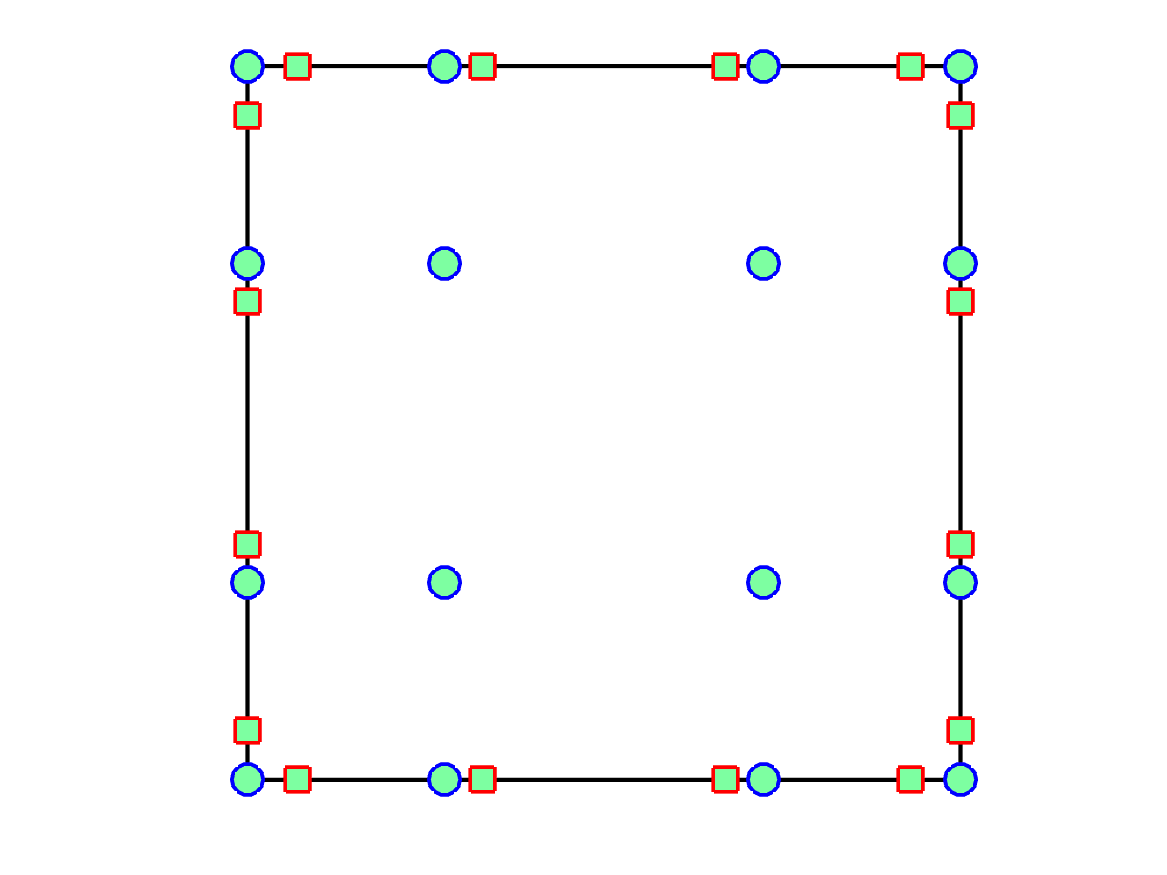
\includegraphics[width=.4\textwidth]{figs/gllgauss.png}\label{subfig:gllgq}}
\hspace{2em}
\subfloat[Degree $2N$ volume quadrature, GLL surface quadrature]{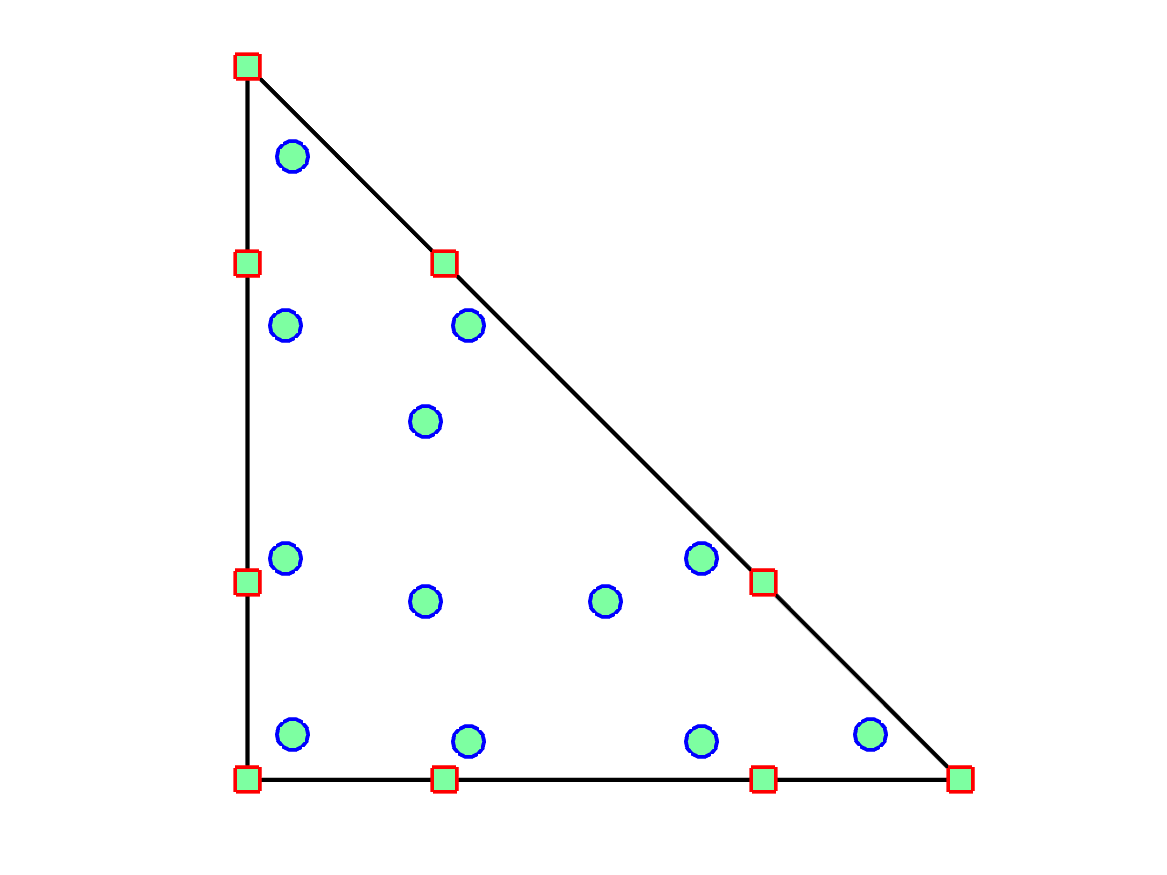
\includegraphics[width=.4\textwidth]{figs/trigll.png}\label{subfig:trigll}}
\caption{Volume and surface quadrature pairs which do not satisfy the assumptions of Lemma~\ref{lemma:dsbp}, and thus do not possess the decoupled SBP property (\ref{eq:dsbp}). }
\label{fig:sbploss}
\end{figure}

\paragraph{Quadrilateral elements (Figure~\ref{subfig:gllgq})} We first consider a quadrilateral element $\hat{D}$ with an $(N+1)$ point tensor product GLL volume quadrature and $(N+1)$ point Gauss quadrature on each face.  Let $u,v \in Q^N$ denote two arbitrary degree $N$ polynomials.  The assumptions of Lemma~\ref{lemma:dsbp} are that the volume quadrature exactly integrates $\int_{\hat{D}} \pd{u}{x} v$ and that the surface quadrature exactly integrates $\int_{\partial \hat{D}} u v n_i$ on $\hat{D}$.  Because the $(N+1)$-point Gauss rule is exact for polynomials of degree $2N+1$ and the product $uv \in P^{2N}$ on each face, the surface quadrature satisfies the assumptions of Lemma~\ref{lemma:dsbp}.  However, the 1D GLL rule is only exact for polynomials of degree $(2N-1)$.  The derivative $\pd{u}{x}$ is a polynomial of degree $(N-1)$ in $x$, but is degree $N$ in $y$.  Thus, $\pd{u}{x}v$ is a polynomial of degree $(2N-1)$ in $x$ but degree $2N$ in $y$, and is not integrated exactly by the volume quadrature.  

\paragraph{Triangular elements (Figure~\ref{subfig:trigll})} We next consider a triangular element $\hat{D}$, where the volume quadrature is exact for degree $2N$ polynomials \cite{xiao2010quadrature} and an $(N+1)$-point GLL quadrature on each face.  Let $u,v \in P^N$ denote two arbitrary degree $N$ polynomials.  The derivative $\pd{u}{x} \in P^{(N-1)}$, and $\pd{u}{x}v \in P^{(2N-1)}$, so the volume quadrature satisfies the assumptions of Lemma~\ref{lemma:dsbp}.  However, because the surface quadrature is exact only degree $(2N-1)$ polynomials and the trace of $uv\in P^{2N}$, the surface quadrature does not satisfy the assumptions of Lemma~\ref{lemma:dsbp}.

\begin{figure}
\centering
\begingroup
\captionsetup[subfigure]{width=.425\textwidth}
\subfloat[Insufficiently accurate surface quadrature on the triangle element.]{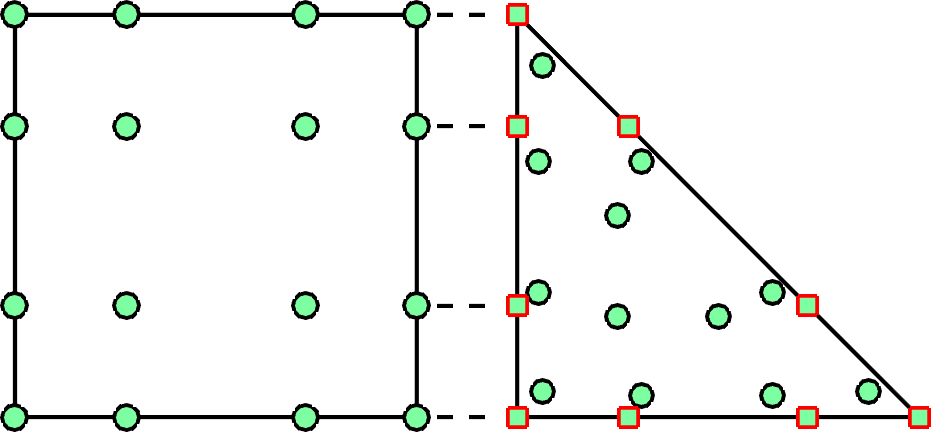
\includegraphics[width=.425\textwidth]{figs/hybrid2D.png}\label{subfig:hybrid1}}
\endgroup
\hspace{2em}
\subfloat[Incompatible surface quadrature on the quadrilateral element.]{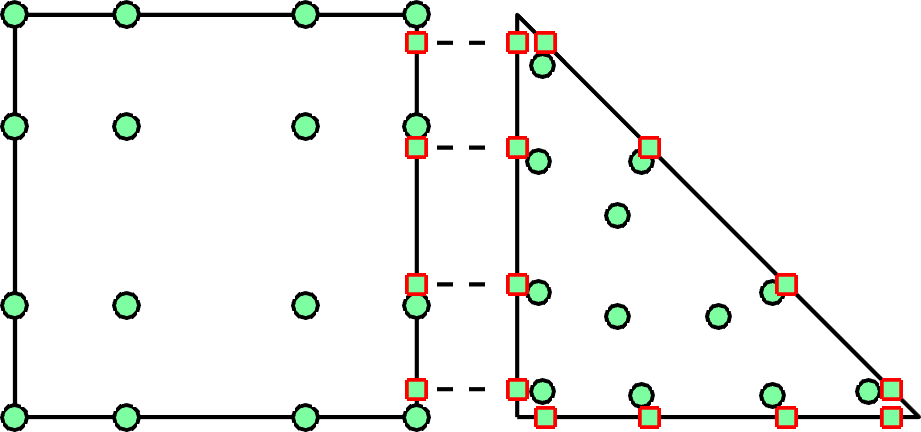
\includegraphics[width=.425\textwidth]{figs/hybrid2D_GQ.png}\label{subfig:hybrid2}}
\caption{Examples of interface couplings which do not result in a decoupled SBP property (\ref{eq:dsbp}).  }
\label{fig:hybrid}
\end{figure}

These specific pairings of volume and surface quadratures appear naturally for hybrid meshes consisting of DG-SEM quadrilateral elements (using GLL volume quadrature) and triangular elements, as shown in Figure~\ref{fig:hybrid}.  In Figure~\ref{subfig:hybrid1}, the surface quadrature is a $(N+1)$ point GLL rule, and results in a loss of the SBP property on the triangle.  In Figure~\ref{subfig:hybrid2}, the surface quadrature is a $(N+1)$ point Gauss-Legendre rule, and results in a loss of the SBP property on the quadrilateral element.  The goal of this work is to construct high order accurate discretizations which preserve entropy conservation for situations in which the decoupled SBP property (\ref{eq:dsbp}) does not hold.  

%\begin{figure}
%\centering
%\subfloat[Hex-pyramid coupling]{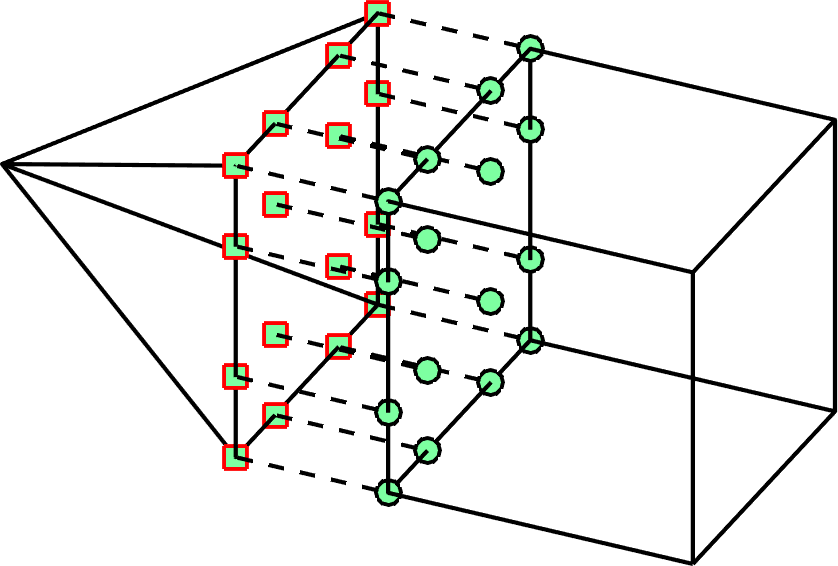
\includegraphics[width=.35\textwidth]{figs/hybrid3D.png}}
%\hspace{2em}
%\subfloat[Hex-prism coupling]{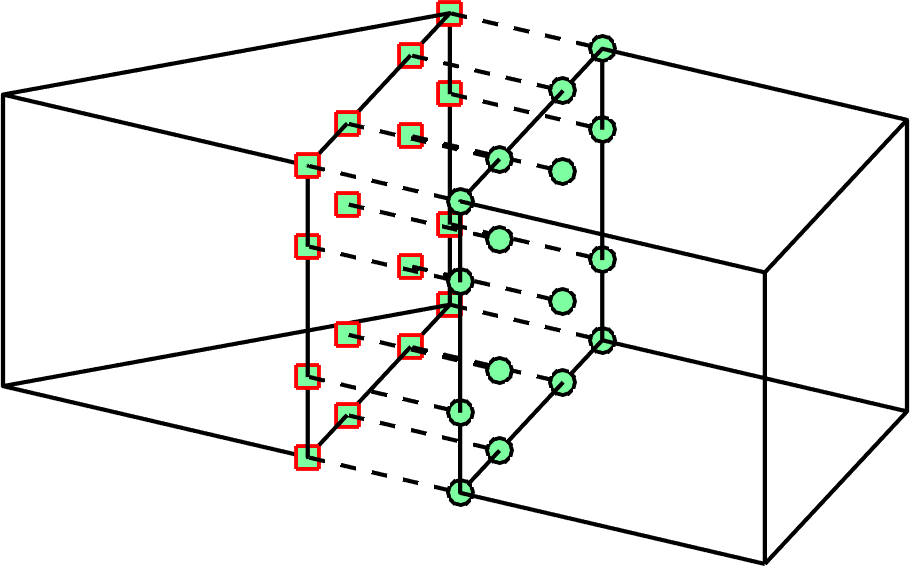
\includegraphics[width=.375\textwidth]{figs/hybrid3D_wedge.png}}
%\caption{Illustration of a 3D coupling between a GLL hexahedral element and a pyramid.  The SBP property does not hold on the pyramid due to the use of GLL quadrature on the quadrilateral face. }
%\label{fig:hybrid3d}
%\end{figure}
%
%\begin{figure}[!h]
%\centering
%\begingroup
%\captionsetup[subfigure]{width=.45\textwidth}
%\subfloat[Entropy stable inter-element coupling in \cite{friedrich2017entropy} for a non-conforming interface.]{\raisebox{0em}{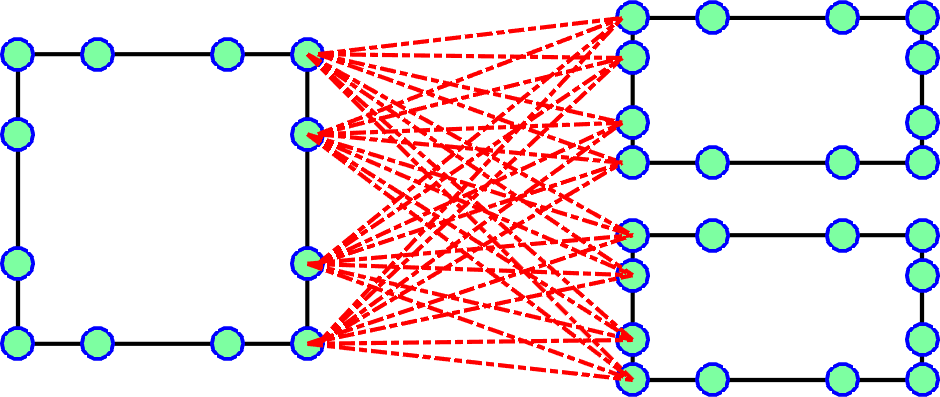
\includegraphics[width=.45\textwidth]{figs/nonconSBP.png}}\label{subfig:noncon2}}
%\hspace{2em}
%\subfloat[Entropy stable inter-element coupling in this work for a non-conforming interface.  The dotted black lines denote communication between neighboring elements.]{\raisebox{-0em}{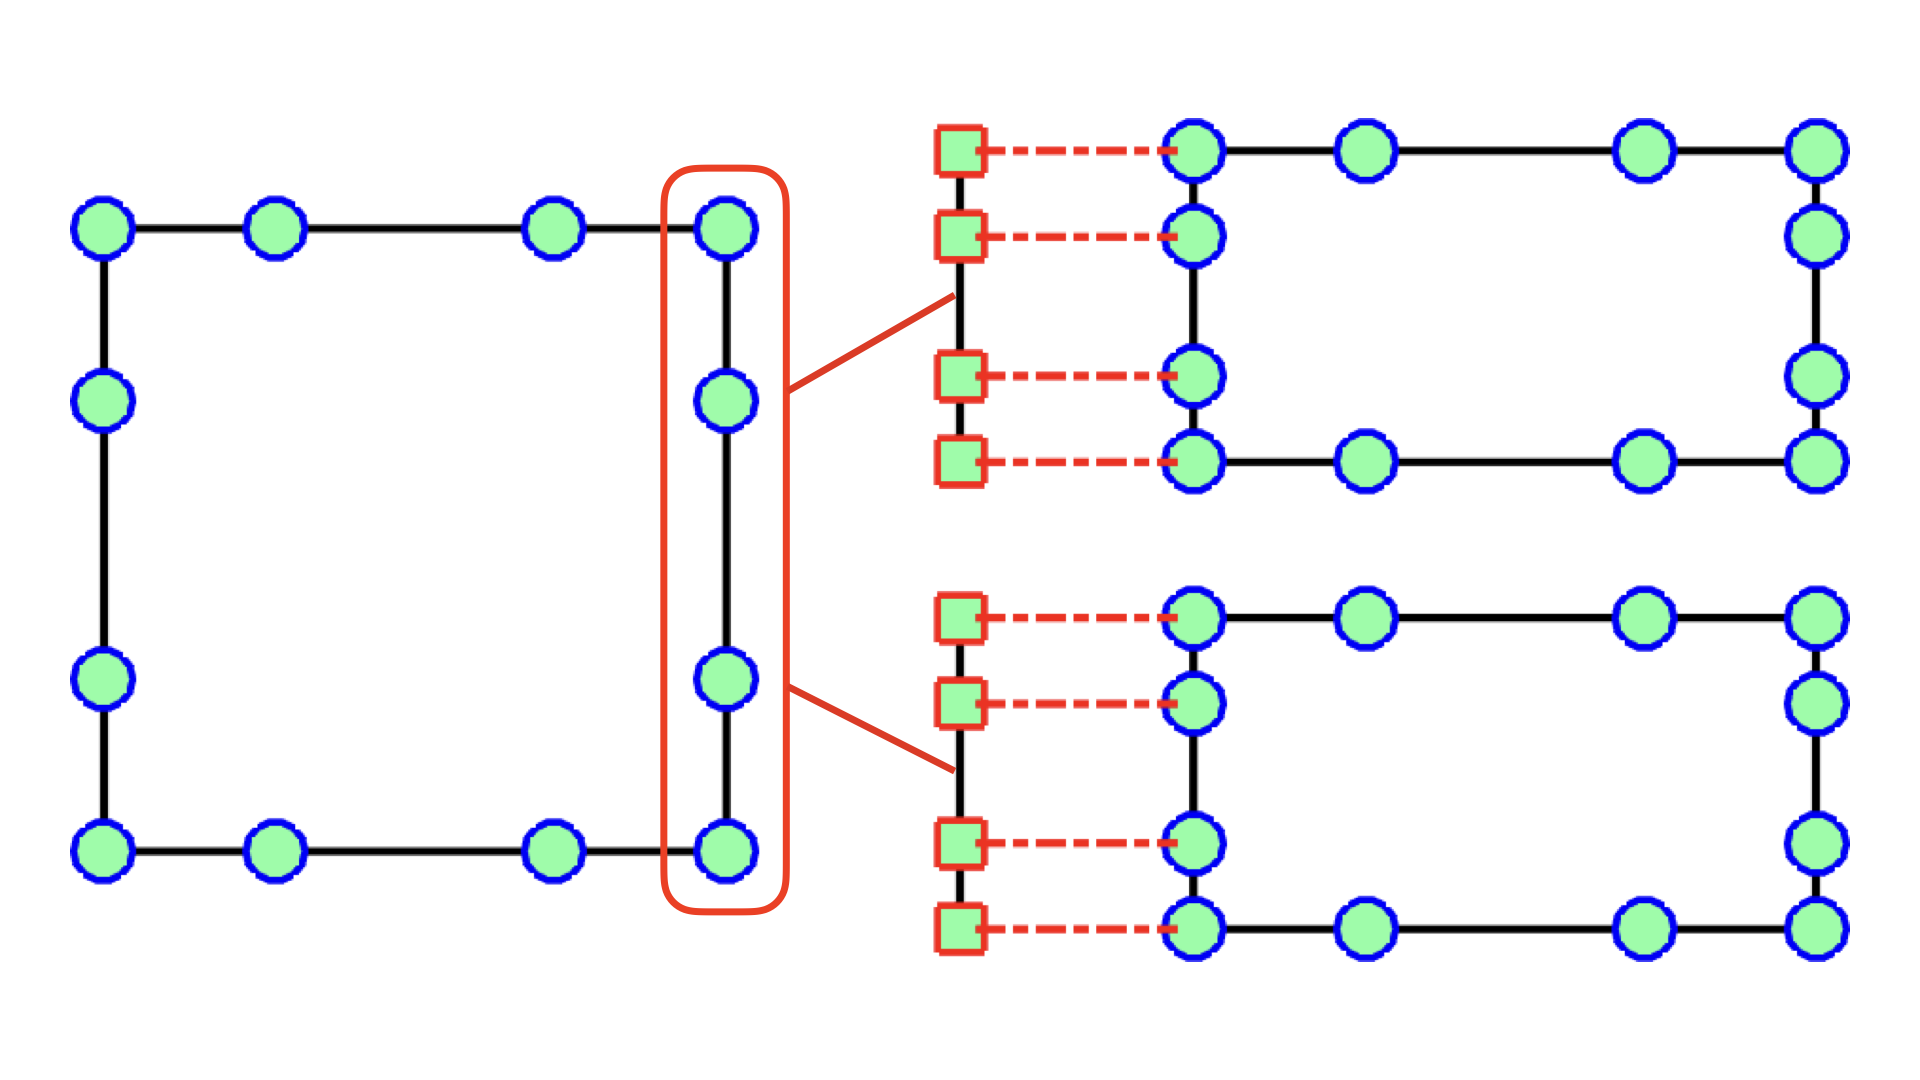
\includegraphics[width=.45\textwidth]{figs/nonconQuad.png}}\label{subfig:noncon1}}
%\endgroup
%%\subfloat[3D hexahedra-pyramid coupling]{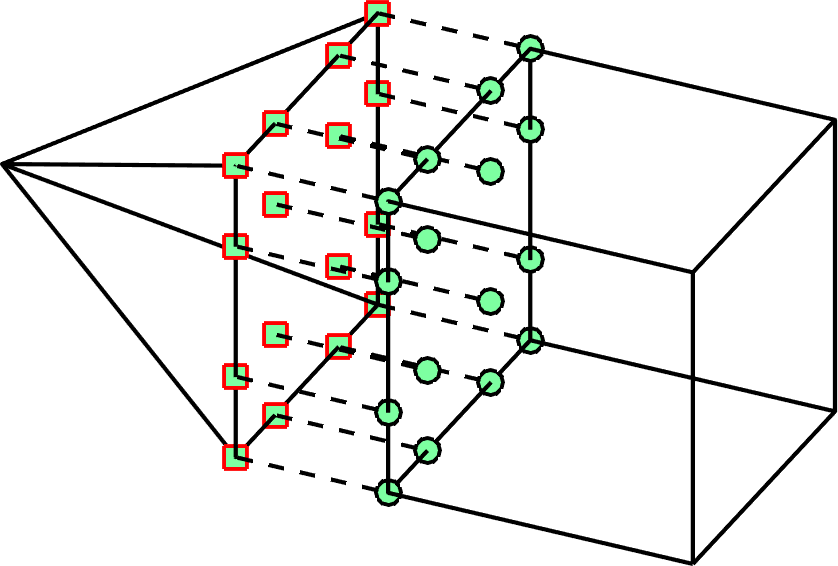
\includegraphics[width=.31\textwidth]{figs/hybrid3D.png}}
%\caption{Illustration of two different entropy stable inter-element couplings for $h$ non-conforming meshes.  Each dashed red line indicates a dyadic flux computation required between two nodes. } %The coupling terms in \cite{friedrich2017entropy} requires computing dyadic fluxes between \emph{each} pair of nodes on adjacent interfaces.  The new approach results in a simpler communication pattern between elements. }
%\label{fig:noncon}
%\end{figure}


\subsection{A variational SBP property}

%The main restriction we wish to overcome 

The property (\ref{eq:dsbp}) (which we will refer to as the ``strong'' SBP property) relates the polynomial exactness of specific quadrature rules to algebraic properties of quadrature-based matrices.  We will relax accuracy conditions on these quadrature rules by utilizing not the strong SBP property, but a weaker ``variational'' version of the SBP property.  This variational property relies on the assumption that the volume and surface quadrature rules are exact for polynomials of certain degrees.  

\begin{assumption}
\label{ass:quad}
Let $v(\bm{x})$ be a polynomial such that $v \in V^{M_{\rm vol}}$ with surface trace $\LRl{v}_{\partial \hat{D}} \in V^{M_{\rm face}}\LRp{f}$ for $f \in \partial \hat{D}$, where $M_{\rm vol}, M_{\rm face} \leq N$ are two non-negative integers.  We assume that the volume and surface quadrature rules are sufficiently accurate such that
\begin{enumerate}
\item the mass matrix $\bm{M}$ is positive definite, 
\item the volume and surface quadratures exactly integrate the quantities $\int_{\hat{D}} \pd{u}{x_i} v$ and $\int_{\partial \hat{D}} u v n_i$ for all $u \in V^N\LRp{\hat{D}}$, $i = 1,\ldots, d$, and $f \in \partial \hat{D}$.  
\end{enumerate}
\end{assumption}

This section presumes that Assumption~\ref{ass:quad} is satisfied for general  $M_{\rm vol}, M_{\rm surf}$.  In Sections~\ref{sec:affine} and \ref{sec:curved}, specific values of $M_{\rm vol}, M_{\rm surf}$ will be motivated by proofs of entropy stability, and Assumption~\ref{ass:quad} will be verified for specific choices of volume and surface quadrature on simplicial and tensor product elements.
%Suppose Assumption~\ref{ass:quad} is satisfied, and let $\bm{v}_q$ denote the vector of values of $v(\bm{x})$ at volume quadrature points.  Then, for an arbitrary vector $\bm{u}_q$, 
%\[
%\bm{v}_q^T \bm{Q}_i \bm{u}_q = \int_{\hat{D}} \pd{u}{x_i} v, \qquad \LRp{\bm{V}_f\bm{P}_q\bm{v}_q}^T\bm{W}_f \diag{\hat{\bm{n}_i}} \bm{V}_f\bm{P}_q\bm{u}_q =  \int_{\partial \hat{D}} \Pi_N u v n_i,
%\]
%where we have used that, because $v$ is a polynomial of degree $N$, it is equal to its own $L^2$ projection.

The conditions in Assumption~\ref{ass:quad} are sufficient to ensure that the following variational SBP property holds:
\begin{lemma}
\label{lemma:vsbp}
%Assume that $v \in V^M$.  
%If the volume quadrature is exact for polynomials of degree $N+M-1$ and the surface quadrature is exact for polynomials of degree $N+M$, 
Suppose Assumption~\ref{ass:quad} holds, and let $\bm{v}_q$ denote the vector of values of $v(\bm{x})$ of at volume quadrature points. Let $u(\bm{x})$ be an $L^2$ integrable function, and let $\bm{u}_q$ denote the values of $u(\bm{x})$ at quadrature points.  Then, 
\[
\bm{v}_q^T\bm{Q}_i \bm{u}_q = \bm{v}_q^T\LRp{ \LRp{\bm{V}_f\bm{P}_q}^T \bm{W}_f \diag{\hat{\bm{n}}_i}\bm{V}_f\bm{P}_q - \bm{Q}_i^T}\bm{u}_q.
\]
\end{lemma}
\begin{proof}
Recall that $\bm{Q}_i = \bm{W} \bm{V}_q \bm{D}^i\bm{P}_q$.  The quadrature-based $L^2$ projection $\Pi_Nu$ is a polynomial of degree $N$, and is computed discretely as $\bm{P}_q\bm{u}_q$.  By the exactness of the volume quadrature in Assumption~\ref{ass:quad}, 
\begin{align*}
\bm{v}_q^T\bm{Q}_i \bm{u}_q &= \bm{v}_q^T\bm{W} \bm{D}^i \bm{P}_q \bm{u}_q = \int_{\hat{D}} \pd{\Pi_N u}{\hat{x}_i} v = \int_{\partial \hat{D}} (\Pi_N u) v \hat{n}_i - \int_{\hat{D}} \LRp{\Pi_N u} \pd{v}{\hat{x}_i}.
\end{align*}
%Since the volume integrand $\LRp{\Pi_N u} \pd{v}{\hat{x}_i} \in V^{N+M-1}$, it is exactly integrated using the volume quadrature.  
%Additionally, since $\Pi_N u \in V^N$ and $v\in V^M$ on the surface of $\hat{D}$, the surface quadrature is exact for the surface integral and 
By the exactness of the surface quadrature in Assumption~\ref{ass:quad}, 
\begin{align*}
&\int_{\partial \hat{D}} (\Pi_N u) v \hat{n}_i -   \int_{\hat{D}} \LRp{\Pi_N u} \pd{v}{\hat{x}_i} =\\
 &\bm{v}_f^T\bm{W}_f{\rm diag}(\hat{\bm{n}}_i) \bm{V}_f\bm{P}_q\bm{u}_q - \LRp{\bm{V}_q\bm{D}^i\bm{P}_q\bm{v}_q}^T\bm{W} \bm{V}_q\bm{P}_q\bm{u}_q\\
=& \bm{v}_q^T \LRp{\bm{V}_f\bm{P}_q}^T\bm{W}_f{\rm diag}(\hat{\bm{n}}_i) \bm{V}_f\bm{P}_q\bm{u}_q - \bm{v}_q^T \bm{P}_q^T\LRp{\bm{D}^i}^T \bm{V}_q^T \bm{W} \bm{V}_q\bm{P}_q\bm{u}_q,
\end{align*}
where we have used that, since $v \in V^N$, $\bm{v}_f = \bm{V}_f\bm{P}_q\bm{v}_q$.  The proof is completed by noting that 
\[
\bm{P}_q^T\LRp{\bm{D}^i}^T \bm{V}_q^T \bm{W} \bm{V}_q\bm{P}_q = \bm{P}_q^T\LRp{\bm{D}^i}^T \bm{M}\bm{P}_q = \bm{P}_q^T\LRp{\bm{D}^i}^T \bm{V}_q^T\bm{W} = \bm{Q}_i^T.
\]
\end{proof}

The variational SBP property in Lemma~\ref{lemma:vsbp} can be used to prove a similar property for the decoupled SBP operator.  This property, along with the exact differentiation of constants, is necessary for the proof of entropy stability.  
\begin{lemma}
Suppose Assumption~\ref{ass:quad} holds.  Let $\bm{D}^i_N$ be a decoupled SBP operator on the reference element $\hat{D}$.  
%Let the volume quadrature be exact for polynomials of degree $N+M-1$, and let the surface quadrature be exact for polynomials of degree $N+M$ for some $M \leq N$.  Suppose $v\in V^N$ and that $\LRl{v}_{\partial \hat{D}} \in P^M\LRp{\partial \hat{D}}$.  \note{Fix this to match assumptions in previous lemma.}
Then, the following variational SBP property holds:
\[
\bm{v}^T\bm{Q}^i_N\bm{u} = \bm{v}^T\LRp{\bm{B}^i_N - \LRp{\bm{Q}^i_N}^T}\bm{u}.%, \qquad \bm{Q}^i_N \bm{1} = \bm{0}.
\]
where $\bm{v}, \bm{u}$ denotes the values of $v$ and $u$ at both volume and surface quadrature points.  
\label{lemma:vdsbp}
\end{lemma}
\begin{proof}
For convenience, let $\bm{u}_q, \bm{u}_f$ and $\bm{v}_q, \bm{v}_f$ denote evaluations of $u$ and $v$ at volume and surface points, such that 
\[
\bm{u} = \begin{pmatrix} \bm{u}_q\\ \bm{u}_f\end{pmatrix}, \qquad \bm{v} = \begin{pmatrix} \bm{v}_q\\ \bm{v}_f\end{pmatrix}.  
\]
The proof of the variational summation by parts property uses the definition of $\bm{Q}^i_N$ (\ref{eq:QN}), 
\begin{align*}
\bm{v}^T\bm{Q}^i_N\bm{u} &= \bm{v}_q^T\bm{Q}_i \bm{u}_q - \frac{1}{2}\LRp{\bm{V}_f\bm{P}_q\bm{v}_q}^T\bm{W}_f\hat{\bm{n}}_i \LRp{\bm{V}_f\bm{P}_q\bm{u}_q} + \frac{1}{2}\LRp{\bm{V}_f\bm{P}_q\bm{v}_q}^T\bm{W}_f\hat{\bm{n}}_i \bm{u}_f\\
& - \frac{1}{2}\bm{v}_f^T\bm{W}_f\hat{\bm{n}}_i \LRp{\bm{V}_f\bm{P}_q\bm{u}_q} + \frac{1}{2}\bm{v}_f^T\bm{W}_f\hat{\bm{n}}_i \bm{u}_f.
\end{align*}
Applying Lemma~\ref{lemma:vsbp} then yields
\begin{align*}
\bm{v}^T\bm{Q}^i_N\bm{u} =& -\bm{v}_q^T\bm{Q}^T_i \bm{u}_q + \frac{1}{2}\LRp{\bm{V}_f\bm{P}_q\bm{v}_q}^T\bm{W}_f\hat{\bm{n}}_i \LRp{\bm{V}_f\bm{P}_q\bm{u}_q} + \frac{1}{2}\LRp{\bm{V}_f\bm{P}_q\bm{v}_q}^T\bm{W}_f\hat{\bm{n}}_i \bm{u}_f\\
&\qquad - \frac{1}{2}\bm{v}_f^T\bm{W}_f\hat{\bm{n}}_i \LRp{\bm{V}_f\bm{P}_q\bm{u}_q} - \frac{1}{2}\bm{v}_f^T\bm{W}_f\hat{\bm{n}}_i \bm{u}_f + \bm{v}_f^T\bm{W}_f\hat{\bm{n}}_i \bm{u}_f\\
=& \begin{pmatrix} \bm{v}_q\\ \bm{v}_f\end{pmatrix}^T 
\left(\begin{pmatrix}
\bm{0}& \\
& \bm{W}_f\diag{\hat{\bm{n}}_i}
\end{pmatrix}\right.\\
&+
\left.\begin{pmatrix}
-\bm{Q}_i^T + \frac{1}{2}\LRp{\bm{V}_f\bm{P}_q}^T\bm{W}_f\hat{\bm{n}}_i \bm{V}_f\bm{P}_q & -\frac{1}{2} \LRp{\bm{W}_f\hat{\bm{n}}_i \bm{V}_f\bm{P}_q}^T\\
\frac{1}{2}\bm{W}_f\hat{\bm{n}}_i \bm{V}_f\bm{P}_q & -\frac{1}{2}\bm{W}_f\hat{\bm{n}}_i
\end{pmatrix}  \right)
\begin{pmatrix} \bm{u}_q\\ \bm{u}_f\end{pmatrix}\\
=& \bm{v}^T\LRp{\bm{B}^i_N - \LRp{\bm{Q}^i_N}^T}\bm{u}.
\end{align*}
\end{proof}

\subsection{Entropy stability on affine meshes}
\label{sec:affine}

In this section, we construct so-called ``entropy stable'' schemes on the reference element $\hat{D}$ and affine meshes.  These methods ensure that the entropy inequality (\ref{eq:entropyineq}) is satisfied discretely by avoiding the use of the chain rule in the proof of entropy dissipation.  Entropy stable schemes rely on two main ingredients: an entropy stable numerical flux as defined by Tadmor \cite{tadmor1987numerical} and a concept referred to as ``flux differencing''.  Let $\bm{f}_S\LRp{\bm{u}_L,\bm{u}_R}$ be a numerical flux function which is a function of ``left'' and ``right'' states $\bm{u}_L,\bm{u}_R$.  The numerical flux $\bm{f}_S$ is \textit{entropy conservative} if it satisfies the following three conditions:  
\begin{gather}
\bm{f}_S(\bm{u},\bm{u}) = \bm{f}(\bm{u}), \qquad \text{(consistency)}\\
\bm{f}_S(\bm{u}_L,\bm{u}_R) = \bm{f}_S(\bm{u}_R,\bm{u}_R), \qquad \text{(symmetry)}\nonumber\\
\LRp{\bm{v}_L-\bm{v}_R}^T\bm{f}_S(\bm{u}_L,\bm{u}_R) = \psi(\bm{u}_L) - \psi(\bm{u}_R), \qquad \text{(conservation)}\nonumber
\label{eq:esflux}
\end{gather}
The construction of entropy stable schemes will utilize (\ref{eq:esflux}) in discretizations of both volume and surface terms in a DG formulation.  

Proving a semi-discrete entropy inequality typically involves the ``strong'' SBP condition.  The schemes presented in this work will relax this, and use only two (weaker) conditions: that the decoupled SBP operator $\bm{D}^i_N$ exactly differentiates constants and that a discrete form of the fundamental theorem of calculus (FTC) holds.  The latter property can be derived from the variational SBP property in Lemma~\ref{lemma:vdsbp}.

\begin{corollary}{(Discrete FTC and exact differentiation of constants)}
\label{lemma:sbpcor}
Suppose Assumption~\ref{ass:quad} holds for $M_{\rm vol} = M_{\rm surf} = 0$ (i.e.\ for $v(\bm{x})$ constant).  
Let $u(\bm{x})$ be some $L^2$ integrable function, and let $\bm{u}$ denote the vector of values of $u(\bm{x})$ at volume and surface quadrature points. Then, 
\[
\bm{1}^T\bm{Q}^i_N\bm{u} = \bm{1}^T\bm{B}^i_N\bm{u}, \qquad \bm{Q}^i_N\bm{1} = \bm{0}.
\]
\end{corollary}
\begin{proof}
The proof that $\bm{Q}^i_N \bm{1} = \bm{0}$ follows from the property that polynomials are equal to their $L^2$ projection, and is identical to that of \cite{chan2017discretely,chan2018discretely}.     The proof of the first equality follows from $\bm{Q}^i_N \bm{1} = \bm{0}$ and Lemma~\ref{lemma:vdsbp} with $M=0$
\[
\bm{1}^T\LRp{\bm{Q}^i_N}\bm{u} = \bm{1}^T\LRp{\bm{B}^i_N - \LRp{\bm{Q}^i_N}^T}\bm{u} = \bm{1}^T{\bm{B}^i_N}\bm{u}.
\]
\end{proof}

We can now construct a skew-symmetric formulation on the reference element $\hat{D}$ and show that it is semi-discretely entropy conservative. We will then extend this formulation to affine elements.  In both cases, this formulation can be made entropy stable by adding interface dissipation.  

Let $\bm{u}_h$ denote the discrete solution, and let $\bm{u}_q$ denote the values of the solution at volume quadrature points.  We define the auxiliary conservative variables $\tilde{\bm{u}}$ in terms of the $L^2$ projections of the entropy variables 
\begin{gather}
\bm{v}_q = \bm{v}\LRp{\bm{u}_q}, \qquad \tilde{\bm{v}} = \begin{bmatrix}
\bm{V}_q\\
\bm{V}_f
\end{bmatrix}\bm{P}_q\bm{v}_q, \qquad \tilde{\bm{u}} = \bm{u}\LRp{\tilde{\bm{v}}}.
\end{gather}
The skew-symmetric formulation for (\ref{eq:nonlineqs}) on $\hat{D}$ is given in terms of $\tilde{\bm{u}}$
\begin{gather}
\bm{M}\pd{\bm{u}_h}{t} + \sum_{i=1}^d\LRs{\begin{array}{c}
\bm{V}_q \\ \bm{V}_f\end{array}}^T 
\LRp{\LRp{\bm{Q}^i_N - \LRp{\bm{Q}^i_N}^T} \circ \bm{F}_S}\bm{1} + \bm{V}_f^T\bm{W}_f \diag{\hat{\bm{n}}_i}\bm{f}_i^* = 0,  \label{eq:esdgSkew}\\
\LRp{\bm{F}_S}_{ij} = \bm{f}_S\LRp{\tilde{\bm{u}}_i,\tilde{\bm{u}}_j}, \qquad 1\leq i,j\leq N_q + N^f_q,\nonumber
\end{gather}
where $\bm{f}^*$ is some numerical flux, and the matrix $\LRp{\bm{Q}^i_N - \LRp{\bm{Q}^i_N}^T}$ possesses the following block structure:
\[
\LRp{\bm{Q}^i_N - \LRp{\bm{Q}^i_N}^T} = \begin{pmatrix}
\bm{Q}_i-\bm{Q}_i^T & \LRp{\bm{V}_f \bm{P}_q}^T\bm{W}_f\diag{\bm{n}_i}\\
-\bm{W}_f\diag{\bm{n}_i}{\bm{V}_f \bm{P}_q} & \bm{0}
\end{pmatrix}.
\]
Multiplying the formulation (\ref{eq:esdgSkew}) by $\bm{M}^{-1}$ on both sides yields a strong form 
\begin{gather}
\pd{\bm{u}_h}{t} + \sum_{i=1}^d \LRs{\begin{array}{cc}
\bm{P}_q & \bm{L}_f\end{array}} \LRp{\LRp{\bm{D}^i_N - \bm{W}_N^{-1}\LRp{\bm{Q}^i_N}^T} \circ \bm{F}_S}\bm{1} + \bm{L}_f \diag{\hat{\bm{n}}_i}\bm{f}_i^* = 0,\label{eq:esdg}
%\\
%\LRp{\bm{F}_S}_{ij} = \bm{f}_S\LRp{\tilde{\bm{u}}_i,\tilde{\bm{u}}_j}, \qquad 1\leq i,j\leq N_q + N^f_q.
%\label{eq:esdgSkewStrong}
\end{gather}
We can now show that the skew-symmetric formulation is entropy conservative.  
\begin{theorem}
Suppose Assumption~\ref{ass:quad} holds for $M_{\rm vol} = M_{\rm surf} = 0$.  
Then, the formulation (\ref{eq:esdgSkew}) is entropy conservative such that
\[
\bm{1}^T\bm{W}\pd{U(\bm{u}_q)}{t} + \sum_{i=1}^d\bm{1}^T\bm{W}_f \diag{\hat{\bm{n}}_i} \LRp{\psi_i(\tilde{\bm{u}}_f) - \tilde{\bm{v}}_f^T\bm{f}_i^*} = 0, \qquad \bm{u}_q = \bm{V}_q\bm{u}.
\]
\label{thm:esdg}
\end{theorem}
\begin{proof}
Testing (\ref{eq:esdgSkew}) by $\bm{v}_h = \bm{P}_q\bm{v}_q$ yields 
\begin{align}
\bm{v}_q^T\bm{W}\pd{\LRp{\bm{V}_q\bm{u}}}{t} + \sum_{i=1}^d
\tilde{\bm{v}}^T \LRp{\LRp{\bm{Q}^i_N - \LRp{\bm{Q}^i_N}^T} \circ \bm{F}_S}\bm{1} + \tilde{\bm{v}}_f^T \bm{W}_f \diag{\hat{\bm{n}}_i}\bm{f}_i^* = 0.
\end{align}
One can show that \cite{chan2017discretely}
\begin{align*}
\tilde{\bm{v}}^T \LRp{\LRp{\bm{Q}^i_N - \LRp{\bm{Q}^i_N}^T} \circ \bm{F}_S}\bm{1} &= \tilde{\bm{v}}^T \LRp{\bm{Q}^i_N \circ \bm{F}_S}\bm{1} - \tilde{\bm{v}}^T \LRp{\LRp{\bm{Q}^i_N}^T \circ \bm{F}_S}\bm{1}\\
&= \tilde{\bm{v}}^T \LRp{\bm{Q}^i_N \circ \bm{F}_S}\bm{1} - \bm{1}^T \LRp{{\bm{Q}^i_N} \circ \bm{F}_S}\tilde{\bm{v}}.
\end{align*}
Where we have used that $\bm{F}_S$ is symmetric and that the Hadamard product commutes.  Applying the conservation condition on $\bm{f}_S$ in (\ref{eq:esflux}) then yields
\begin{align*}
\tilde{\bm{v}}^T \LRp{\bm{Q}^i_N \circ \bm{F}_S}\bm{1} - \bm{1}^T \LRp{{\bm{Q}^i_N} \circ \bm{F}_S}\tilde{\bm{v}} &= \sum_{jk} \LRp{\bm{Q}^i_N}_{jk} \LRp{\tilde{\bm{v}}_j-\tilde{\bm{v}}_k} \bm{f}_S\LRp{\tilde{\bm{u}}_j,\tilde{\bm{u}}_k} \\
&= \sum_{ij} \LRp{\bm{Q}^i_N}_{jk} \LRp{\psi_i(\tilde{\bm{u}}_j) - \psi_i(\tilde{\bm{u}}_k)}\\
&= \bm{1}^T\LRp{\bm{Q}^i_N}\psi_i(\tilde{\bm{u}}) - \psi_i(\tilde{\bm{u}})^T\LRp{\bm{Q}^i_N}\bm{1} \\
&= \bm{1}^T\LRp{\bm{Q}^i_N}\psi_i(\tilde{\bm{u}}) = \bm{1}^T\bm{B}^i_N\psi_i(\tilde{\bm{u}}),
\end{align*}
where we have used Corollary~\ref{lemma:sbpcor} in the last equality.  Noting that $\bm{1}^T\bm{B}^i_N\psi_i(\tilde{\bm{u}}) = \bm{1}^T\bm{W}_f \diag{\hat{\bm{n}}_i} \psi_i(\tilde{\bm{u}}_f)$ completes the proof.
%The final step of the proof is  where we have used Lemma~\ref{lemma:vdsbp} to integrate by parts and conclude that $\bm{1}^T\LRp{\bm{Q}^i_N}^T = 0$.
\end{proof}

\begin{remark}
It should be emphasized that the only result necessary to prove Theorem~\ref{thm:esdg} is Corollary~\ref{lemma:sbpcor}.  The decoupled SBP property (\ref{eq:dsbp}) is not utilized, and is not necessary to guarantee a semi-discrete conservation of entropy.  
\end{remark}

The skew symmetric formulation can also be shown to be locally conservative in the sense of \cite{shi2017local}, which is sufficient to show the numerical solution convergences to the weak solution under mesh refinement.  
\begin{theorem}
The formulation (\ref{eq:esdgSkew}) is locally conservative such that
\begin{align}
\bm{1}^T\bm{W}\pd{\LRp{\bm{V}_q\bm{u}}}{t} + \sum_{i=1}^d\bm{1}^T\bm{W}_f \diag{\hat{\bm{n}}_i}\bm{f}_i^* = 0. 
\end{align}
\end{theorem}
\begin{proof}
To show local conservation, we test (\ref{eq:esdgSkew}) with $1$
\begin{align}
\bm{1}^T\bm{W}\bm{V}_q\pd{\bm{u}_h}{t} + \sum_{i=1}^d
\bm{1}^T
\LRp{\LRp{\bm{Q}^i_N - \LRp{\bm{Q}^i_N}^T} \circ \bm{F}_S}\bm{1} + \bm{1}^T\bm{W}_f \diag{\hat{\bm{n}}}\bm{f}_i^* = 0. 
\end{align}
Because $\bm{F}_S$ is symmetric and $\LRp{\bm{Q}^i_N - \LRp{\bm{Q}^i_N}^T}$ is skew-symmetric, the term 
\[
\LRp{\LRp{\bm{Q}^i_N - \LRp{\bm{Q}^i_N}^T} \circ \bm{F}_S}
\]
is a skew-symmetric matrix.  Using that $\bm{x}^T\bm{A}\bm{x} = 0$ for any skew symmetric matrix $\bm{A}$, the volume term vanishes
\[
\bm{1}^T\LRp{\LRp{\bm{Q}^i_N - \LRp{\bm{Q}^i_N}^T} \circ \bm{F}_S}\bm{1} = 0.
\]
% and that the Hadamard product is commutable $\LRp{\bm{A}\circ\bm{B} }^T = \bm{A}^T\circ\bm{B}^T$
%\begin{align}
%\bm{1}^T\LRp{\LRp{\bm{Q}^i_N - \LRp{\bm{Q}^i_N}^T} \circ \bm{F}_S}\bm{1} &= \bm{1}^T\LRp{\bm{Q}^i_N\circ \bm{F}_S}\bm{1} - \bm{1}^T\LRp{\LRp{\bm{Q}^i_N}^T\circ \bm{F}_S}\bm{1}\\
%&= \bm{1}^T\LRp{\bm{Q}^i_N\circ \bm{F}_S}\bm{1} - 
%\bm{1}^T\LRp{\bm{Q}^i_N\circ \bm{F}_S}\bm{1} = 0,
%\end{align}
%where we have used that $\bm{F}_S$ is symmetric.
%\begin{align}
%\end{align}
\end{proof}

Next, we extend this formulation to affinely mapped elements.  Let the domain be decomposed into non-overlapping elements $D^k$, such that $D^k$ is the image of the reference element $\hat{D}$ under an affine mapping $\bm{\Phi}^k$.  We define geometric terms ${G}^k_{ij}$ as scaled derivatives of reference coordinates $\hat{\bm{x}}$ w.r.t.\ physical coordinates $\bm{x}$
\begin{gather}
\pd{u}{x_i} = \sum_{ij} {G}^k_{ij}\pd{u}{\hat{x}_j}, \qquad {G}^k_{ij} = J^k\pd{\hat{x}_j}{{x}_i}, 
\label{eq:geofacs}
\end{gather}
where $J^k$ is the determinant of the Jacobian of the geometric mapping on the element $D^k$.  We also introduce the scaled outward normal components $n_iJ^k_f$, which can be computed in terms of (\ref{eq:geofacs}) and the reference normals $\hat{\bm{n}}$ on $\hat{D}$
\begin{gather}
n^k_i J^k_f = \sum_{j=1}^d G^k_{ij} \hat{{n}}_j.  
\label{eq:normals}
\end{gather}
 
Derivatives with respect to physical coordinates on $D^k$ are computed in terms of a change of variables formula and geometric terms (\ref{eq:geofacs}).  For affine meshes, the scaled geometric terms ${G}^k_{ij}$ are constant over each element.  It was shown in \cite{chan2017discretely} that one can define a physical differentiation matrix as a linear combination of reference differentiation matrices.  Let ${\bm{D}}^i_N$ denote the decoupled SBP operator on the reference element $\hat{D}$.  Define the decoupled SBP operators $\bm{D}^i_k$ with respect to the physical coordinates on $D^k$ be defined as
\begin{align}
{\bm{D}}^i_k = \sum_{j=1}^d {G}^k_{ij}{\bm{D}}^j_N.
\end{align}
Let $\bm{n}^k_i$ be a vector containing concatenated values of the scaled outward normals $n^k_iJ^k_f$ at surface quadrature nodes.  
Then, an entropy conservative formulation can be given on $D^k$ as follows:
\begin{gather}
J^k\bm{M}\pd{\bm{u}_h}{t} + 
\sum_{i=1}^d \LRs{\begin{array}{cc}
\bm{V}_q \\
\bm{V}_f\end{array}}^T \LRp{\LRp{\bm{Q}^i_k - \LRp{\bm{Q}^i_k}^T} \circ \bm{F}_S}\bm{1} + \bm{V}_f^T\bm{W}_f \diag{{\bm{n}^k_i}}\bm{f}_i^* = 0, \label{eq:skewform}\\
%\sum_{i=1}^d \LRs{\begin{array}{cc}
%\bm{P}_q & \bm{L}_f\end{array}} \LRp{\LRp{\bm{D}^i_N - \bm{W}_N^{-1}\LRp{\bm{Q}^i_N}^T} \circ \bm{F}_S}\bm{1} + \bm{L}_f \diag{{\bm{n}_i}}\bm{f}_i^* = 0, \label{eq:skewform}\\
\LRp{\bm{F}_S}_{ij} = \bm{f}_S\LRp{\tilde{\bm{u}}_i,\tilde{\bm{u}}_j}, \qquad 1\leq i,j\leq N_q + N^f_q, \nonumber\\
\bm{f}^* = \bm{f}_S(\tilde{\bm{u}}_f^+,\tilde{\bm{u}}_f), \qquad \text{ on interior interfaces,} \nonumber
\end{gather}
where $\tilde{\bm{u}}_f^+$ denotes the face value of the entropy-projected conservative variables $\tilde{\bm{u}}_f$ on the neighboring element.  The entropy conservative formulation can be made entropy stable by adding appropriate interface dissipation, such as Lax-Friedrichs or matrix-based penalization terms \cite{winters2017uniquely, chen2017entropy, chan2017discretely}.  

\subsubsection{On conditions for Assumption~\ref{ass:quad}}

Apart from algebraic manipulations, only Corollary~\ref{lemma:sbpcor} is necessary to prove entropy conservation for (\ref{eq:esdg})  and (\ref{eq:skewform}).  Corollary~\ref{lemma:sbpcor} requires that Assumption~\ref{ass:quad} holds for $M_{\rm vol}=M_{\rm surf}=0$.  Thus, the volume and surface quadratures must be sufficiently accurate to guarantee that the mass matrix is positive definite and to integrate 
\begin{equation}
\int_{\hat{D}} \pd{u}{x_i}, \qquad \int_{\partial \hat{D}} u n_i. \label{eq:affineints}
\end{equation}
On simplicial elements, the mass matrix is guaranteed to be positive definite for any volume quadrature which is exact for degree $2N$ polynomial integrands.  This choice of volume quadrature also guarantees that the volume term in (\ref{eq:affineints}) is integrated exactly.  The surface quadrature can thus be taken to be any quadrature rule which is exact for only degree $N$ integrands on faces.  In contrast, the construction of simplicial SBP operators has generally required face quadratures which are accurate for degree $2N$ polynomials \cite{hicken2016multidimensional, crean2018entropy, chan2018discretely}.  

On tensor product elements, we consider isotropic quadrature rules which are tensor products of one-dimensional quadrature rules.  For example, we can use a quadrature rule constructed through a tensor product of one-dimensional $(N+1)$-point GLL quadrature rules, which is sufficient to guarantee that the mass matrix is positive definite \cite{canuto2007spectral}.  This quadrature rule is also exact for integrands in $Q^{2N-1}$, and thus exactly integrates the volume term in (\ref{eq:affineints}).  This leaves the surface quadrature, which can again be taken to be any quadrature rule exact for degree $N$ integrands.  For example, on a quadrilateral element, one can use either $\left\lceil\frac{N+1}{2}\right\rceil$-point Gauss quadrature rule or a $\left\lceil\frac{N+3}{2}\right\rceil$-point GLL rule as face quadratures for a degree $N$ scheme.
%This minimal degree of surface quadrature accuracy will depend on the nature of the physical mesh, and will differ between affine and curved elements.  


\subsection{Entropy stability on curvilinear meshes}
\label{sec:curved}

On affine meshes, it is possible to show entropy stability of the skew-symmetric formulation (\ref{eq:esdgSkew}) under a surface quadrature which is only exact for degree $N$ polynomials.  However, on curved meshes, stronger conditions are required to guarantee entropy stability.  This is due to the fact that the geometric terms are now high order polynomials which vary spatially over each element.  Moreover, Corollary~\ref{lemma:sbpcor} assumes affine geometric mappings, and does not hold on curved elements.  In this section, we discuss how to extend Corollary~\ref{lemma:sbpcor} to curved simplicial and tensor product elements.  

\subsection{Discrete geometric conservation law and surface quadrature accuracy}

Let the domain now be triangulated by a watertight mesh (as defined in \cite{chan2018discretely}) consisting of curved elements $D^k$.  
In contrast to the affine case, geometric terms $G^k_{ij}$ for a curved element are now high order polynomials over the reference domain $\hat{D}$.  We assume that the scaled normals are still computed from $G^k_{ij}$ using (\ref{eq:normals}).  In this section, we describe how to construct appropriate decoupled SBP operators on curved meshes, and give conditions on the volume and surface quadrature rules under which a semi-discretely entropy stable scheme can be constructed.

We first show how to construct decoupled SBP operators on curved elements.  Let $\bm{G}^k_{ij}$ denote the vector of scaled geometric terms ${G}^k_{ij}$ evaluated at both volume and surface quadrature points.  Decoupled SBP operators on a curved element $D^k$ can be defined as in \cite{chan2018discretely} by
\begin{equation}
\bm{D}^i_k = \frac{1}{2}\sum_{j=1}^d \LRp{\diag{\bm{G}^k_{ij}}{\bm{D}}^j_N + {\bm{D}}^j_N\diag{\bm{G}^k_{ij}}}, \qquad \bm{Q}^i_k = \bm{W} \bm{D}^i_k.
\label{eq:dncurved}
\end{equation}
It can be shown that, if $\bm{D}^j_N$ satisfies a strong summation by parts property, $\bm{D}^i_k$ satisfies an analogous strong summation by parts property.
%The construction of $\bm{D}^i_k$ in (\ref{eq:dncurved}) 
The skew-symmetric formulation (\ref{eq:skewform}) can be extended to curvilinear meshes by replacing the reference element operators $\bm{Q}^i_N$ with the physical operators $\bm{Q}^i_k$ defined by (\ref{eq:dncurved}).  However, additional assumptions must be satisfied in order to prove that the resulting formulation is entropy stable.  

The first assumption which must be satisfied is the discrete geometric conservation law (GCL) \cite{thomas1979geometric, kopriva2006metric}.  For curved elements, Lemma~\ref{lemma:vdsbp} and Corollary~\ref{lemma:sbpcor} do not necessarily hold at the discrete level.  For example, expanding out the condition $\bm{Q}^i_k\bm{1} = \bm{0}$ in terms of (\ref{eq:dncurved}) yields
\begin{align}
\bm{Q}^i_k \bm{1} = \frac{1}{2} \bm{W}\sum_{j=1}^d \diag{\bm{G}^k_{ij}}{\bm{D}}^j_N \bm{1} + {\bm{D}}^j_N\diag{\bm{G}^k_{ij}}\bm{1} = \frac{1}{2}\bm{W}\sum_{j=1}^d {\bm{D}}^j_N\LRp{\bm{G}^k_{ij}} = 0,
\label{eq:dgcl}
\end{align}
where we have used that ${\bm{D}}^j_N \bm{1} = 0$.  For degree $N$ isoparametric mappings, the GCL is automatically satisfied in two dimensions due to the fact that the exact geometric terms ${G}^k_{ij}$ are polynomials of degree $N$ \cite{kopriva2006metric}.  However, in three dimensions, the GCL is not automatically satisfied due to the fact that the degree of $G^k_{ij}$ is larger than $N$.  Thus, the geometric terms cannot be represented exactly using degree $N$ polynomials, and (\ref{eq:dgcl}) must be enforced through an alternative construction of ${G}^k_{ij}$.  

A common approach is to rewrite the geometric terms as the curl of some quantity $\bm{r}^i$, but to interpolate $\bm{r}^i$ before applying the curl \cite{visbal2002use, kopriva2006metric, hindenlang2012explicit}:
\begin{align}
\bm{r}^i = { \pd{\bm{x}}{\hat{x}_i}\times \bm{x}}, \qquad
\LRs{\begin{array}{c}
\bm{G}^k_{i1}\\
\bm{G}^k_{i2}\\
\bm{G}^k_{i3}\end{array}} = -\frac{1}{2}\LRp{\pd{I_{N_{\rm geo}}\bm{r}^k}{\hat{x}_j}-\pd{I_{N_{\rm geo}}\bm{r}^j}{\hat{x}_k}}, 
\label{eq:iconscurl}
\end{align}
where $I_{N_{\rm geo}}$ denotes a degree $N_{\rm geo}$ polynomial interpolation operator with appropriate interpolation nodes.\footnote{This interpolation step must be performed using interpolation points with an appropriate number of nodes on each boundary \cite{chan2018discretely}.  These include, for example, GLL nodes on tensor product elements, as well as Warp and Blend nodes on non-tensor product elements \cite{warburton2006explicit, chan2015comparison}.}  

Because the decoupled SBP operators $\bm{D}^i_k$ are now defined through (\ref{eq:dncurved}), Corollary~\ref{lemma:sbpcor} and the proof of entropy stability no longer hold for curved elements and must be modified.  The introduction of curvilinear meshes will impose slightly different conditions on the accuracy of the surface quadrature.  We discuss simplicial and tensor product elements separately, as differences in the natural polynomial approximation spaces will result in different assumptions for each proof.

\begin{lemma}{(Triangles and tetrahedra)}
Let $D^k$ be a curved simplicial element, and let the geometric terms $G^k_{ij}$ be constructed .  If the volume quadrature is exact for polynomials of degree $(N+N_{\rm geo}-1)$ and the surface quadrature is exact for polynomials of degree $(N+N_{\rm geo})$, then 
\[
\bm{1}^T\bm{Q}^i_k\bm{u} = \bm{1}^T\bm{B}^i_k\bm{u}, \qquad \bm{Q}^i_k\bm{1} = \bm{0}.
\]
where $\bm{u}$ is a vector of values of some function at volume and surface quadrature points. 
\end{lemma}
\begin{proof}
d
\end{proof}


\begin{lemma}{(Quadrilaterals and hexahedra)}
Let $D^k$ be a curved tensor product element.  Then, 
\end{lemma}
\begin{proof}
\note{Proof relies on two facts: that geometric terms are products of }
\end{proof}

%, which are summarized in the following curved version of Corollary~\ref{lemma:sbpcor}.
%\note{Maybe provide 2 lemmas - one for triangles and one for quadrilaterals?  Polynomial degree of geofacs is slightly different between the two.  } 
%\begin{lemma}
%Assume that the geometric terms $\bm{G}^k_{ij} \in V^{N_{\rm geo}}$ satisfy the discrete GCL (\ref{eq:dgcl}), that the volume quadrature is exact for polynomials of degree $N+N_{\rm geo}-1$, and that the surface quadrature is exact for polynomials of degree $N+N_{\rm geo}$.  Then, 
%\[
%\bm{1}^T\bm{Q}^i_k\bm{u} = \bm{1}^T\bm{B}^i_k \bm{u}, 
%\qquad \bm{Q}^i_k \bm{1} = 0, 
%\]
%where 
%\[
%\bm{B}^i_k =  \begin{pmatrix}
%\bm{0}&\\
%& \bm{W}_f \diag{{\bm{n}^k_i}}
%\end{pmatrix}.
%\]
%\label{lemma:vdsbpcurved}
%\end{lemma}
%\begin{proof}
%The second equality $\bm{Q}^i_k \bm{1} = 0$ is a consequence of the discrete GCL (\ref{eq:dgcl}), and the proof is identical to that of \cite{chan2018discretely}.  
%%For the first equality, if the surface quadrature is exact for polynomials of degree $2N$ on the trace space, then the matrix SBP property $\bm{Q}^i_N = \bm{B}^i_N - \LRp{\bm{Q}^i_N}^T$ holds \cite{chan2018discretely}.  Combining this with $\bm{Q}^i_k\bm{1} = 0$ yields the desired result.  We focus on the proof of the variational SBP property for surface quadrature which are exact for polynomials of degree $N+R < 2N$.  
%For the first equality, we utilize the variational SBP property.  
%Expanding $\bm{1}^T\bm{Q}^i_k\bm{u}$ yields
%\[
%\bm{1}^T\bm{Q}^i_k\bm{u} = \frac{1}{2}\sum_{j=1}^d \bm{1}^T \diag{\bm{G}^k_{ij}} {\bm{Q}}^j_N \bm{u} + \bm{1}^T{\bm{Q}}^j_N \diag{\bm{G}^k_{ij}} \bm{u}. %=  \frac{1}{2}\sum_{j=1}^d \bm{1}^T \diag{\bm{G}_{ij}} \hat{\bm{Q}}^j_N \bm{u},
%\]
%For the latter term in the sum, Lemma~\ref{lemma:vdsbp} holds and
%\begin{align}
%\sum_{j=1}^d\bm{1}^T{\bm{Q}}^j_N \diag{\bm{G}^k_{ij}} \bm{u} &= 
%\sum_{j=1}^d\bm{1}^T\LRp{{\bm{B}}^j_N - \LRp{{\bm{Q}}^j_N}^T} \diag{\bm{G}^k_{ij}} \bm{u} \\
%&= \sum_{j=1}^d\bm{1}^T{\bm{B}}^j_N\diag{\bm{G}^k_{ij}}\bm{u}, \nonumber
%\label{eq:vsbp1}
%\end{align}
%where we have used that ${\bm{Q}}^j_N \bm{1} = \bm{0}$.  
%
%For the former term in the sum, we use the fact that $G^k_{ij}$, when constructed using (\ref{eq:iconscurl}), is a polynomial of degree $N$.  Thus, $\bm{G}^k_{ij} = \begin{bmatrix}\bm{V}_q\\ \bm{V}_f\end{bmatrix}\bm{g}$ for some vector of polynomial coefficients $\bm{g}$.  We can then rewrite the former term as
%\begin{gather}
%\sum_{j=1}^d\bm{1}^T \diag{\bm{G}^k_{ij}} {\bm{Q}}^j_N \bm{u} = 
%\sum_{j=1}^d{\bm{G}^k_{ij}}^T {\bm{Q}}^j_N \bm{u}.% = \sum_{j=1}^d \bm{g}^T \begin{bmatrix}\bm{V}_q\\ \bm{V}_f\end{bmatrix}^T{\bm{Q}}^j_N \bm{u}.
%%= \sum_{j=1}^d\begin{bmatrix}
%%\bm{G}^q_{ij}\\
%%\bm{G}^f_{ij}
%%\end{bmatrix}^T \begin{bmatrix} 
%%\hat{\bm{Q}}_i - \frac{1}{2}\LRp{\bm{V}_f \bm{P}_q}^T  \bm{W}_f{\rm diag}(\hat{\bm{n}}_i) \bm{V}_f\bm{P}_q &  \frac{1}{2}\LRp{\bm{W}_f{\rm diag}(\hat{\bm{n}}_i)\bm{V}_f\bm{P}_q}^T\label{eq:ibpg}\\
%%-\frac{1}{2}\bm{W}_f{\rm diag}(\hat{\bm{n}}_i)\bm{V}_f\bm{P}_q & \frac{1}{2}\bm{W}_f{\rm diag}(\hat{\bm{n}}_i)
%%\end{bmatrix} \begin{bmatrix}\bm{u}_q\\
%%\bm{u}_f\end{bmatrix}.\nonumber
%\end{gather}
%%where $\bm{G}^q_{ij},\bm{G}^f_{ij}$ denote the values of $\bm{G}_{ij}$ at volume and surface quadrature points.  
%%Because $\bm{P}_q\bm{V}_q = \bm{I}$, straightforward computations give that %simplify the final expression 
%%\[
%%\begin{bmatrix}\bm{V}_q\\ \bm{V}_f\end{bmatrix}^T{\bm{Q}}^j_N = \begin{bmatrix}
%%\bm{Q}^i-\bm{V}_f^T\bm{W}_f\diag{\hat{\bm{n}}_j}\bm{V}_f\bm{P}_q & \bm{V}_f^T\bm{W}_f\diag{\hat{\bm{n}}_j}
%%\end{bmatrix}
%%\]
%
%Because $\bm{G}_{ij} \in V^N$, it is equal to its own $L^2$ projection, and the values at volume and surface quadrature points are related by $\bm{G}^f_{ij} = \bm{V}_f\bm{P}_q\bm{G}^q_{ij}$.  We can use this to simplify (\ref{eq:ibpg})
%\begin{align*}
%\bm{1}^T \diag{\bm{G}_{ij}} \hat{\bm{Q}}^j_N \bm{u} =&  \LRp{\bm{G}^q_{ij}}^T { \bm{Q}_i}  \bm{u}_q - \frac{1}{2} \LRp{{\bm{V}_f \bm{P}_q}\bm{G}_{ij}^q+\bm{G}^f_{ij}}^T{\bm{W}_f{\rm diag}({\bm{n}}_i)\bm{V}_f\bm{P}_q}\bm{u}_q\\
%&+ \frac{1}{2} \LRp{{\bm{V}_f \bm{P}_q}\bm{G}_{ij}^q+\bm{G}^f_{ij}}^T\frac{1}{2}\bm{W}_f{\rm diag}({\bm{n}}_i)\bm{u}_f\\
%=& \LRp{\bm{G}^q_{ij}}^T \LRp{ \hat{\bm{Q}}_i - \LRp{{\bm{V}_f \bm{P}_q}\bm{G}_{ij}^q}^T{\bm{W}_f{\rm diag}(\hat{\bm{n}}_i)\bm{V}_f\bm{P}_q}}\bm{u}_q \\
%&+ \LRp{\bm{G}^f_{ij}}^T\bm{W}_f{\rm diag}(\hat{\bm{n}}_i)\bm{u}_f. %\\
%%&= \LRp{\bm{G}^q_{ij}}^T \LRp{ \LRp{{\bm{V}_f \bm{P}_q}\bm{G}_{ij}^q}^T{\bm{W}_f{\rm diag}({\bm{n}}_i)\bm{V}_f\bm{P}_q}}\bm{u}_q + \LRp{\bm{G}^f_{ij}}^T\bm{W}_f{\rm diag}({\bm{n}}_i)\bm{u}_f 
%\end{align*}
%The first term can be further simplified using Lemma~\ref{lemma:vsbp}
%\[
%\LRp{\bm{G}^q_{ij}}^T \LRp{ \hat{\bm{Q}}_i - \LRp{{\bm{V}_f \bm{P}_q}\bm{G}_{ij}^q}^T{\bm{W}_f{\rm diag}(\hat{\bm{n}}_i)\bm{V}_f\bm{P}_q}}\bm{u}_q = \LRp{\bm{G}^q_{ij}}^T \LRp{ \hat{\bm{Q}}_i}^T\bm{u}_q.
%\]
%The latter term can be combined with the surface term of (\ref{eq:vsbp1}) by noting that 
%\[
%\LRp{\bm{G}^f_{ij}}^T\bm{W}_f \diag{\hat{\bm{n}}_i}\bm{u}_f =\bm{1}^T\hat{\bm{B}}^j_N\diag{\bm{G}_{ij}}\bm{u} = \bm{1}^T\diag{\bm{G}_{ij}}\hat{\bm{B}}^j_N\bm{u},
%\]
%where we have used that $\hat{\bm{B}}^j_N$ is diagonal and commutes with diagonal scaling by $\bm{G}_{ij}$.
%%as $\LRp{\bm{G}^f_{ij}}^T\bm{W}_f{\rm diag}({\bm{n}}_i)\bm{u}_f = \bm{1}^T\hat{\bm{B}}^j_N \bm{u}$.  
%We can use polynomial exactness and the fact that the geometric terms satisfy the continuous GCL by construction \cite{chan2018discretely} to show that $\sum_{j=1}^d  \hat{\bm{Q}}_j {\bm{G}^q_{ij}} = 0$.
%Combining this with (\ref{eq:vsbp1}) and expanding out $\hat{\bm{B}}^j_N$ yields that
%\begin{align*}
%\bm{1}^T\bm{Q}^i_N\bm{u} &= \sum_{j=1}^d \LRp{
%\frac{1}{2}\LRp{\bm{G}^q_{ij}}^T \LRp{ \hat{\bm{Q}_i}}^T \bm{u}_q + \bm{1}^T\begin{pmatrix}
%\bm{0} &\\
%& \bm{W}_f \diag{\bm{G}_{ij} \circ \hat{\bm{n}}_j}
%\end{pmatrix}
%\bm{u}} \\
%&=  \bm{1}^T\begin{pmatrix}
%\bm{0} &\\
%& \bm{W}_f \diag{\sum_{j=1}^d \bm{G}_{ij} \circ \hat{\bm{n}}_j}
%\end{pmatrix}
%\bm{u} = \bm{1}^T\bm{B}^i_N\bm{u}.
%\end{align*}
%where we have used in the final step that $\sum_{j=1}^d\bm{G}_{ij}\hat{n}_j = \bm{n}_i J^k_f$ \cite{ciarlet1978finite, chan2018discretely}
%\end{proof}

Lemma~\ref{lemma:vdsbpcurved} implies that the polynomial degree $R$ of the surface geometric terms must be compatible with the accuracy of the surface quadrature.  This, in turn, depends on the polynomial degree $N_{\rm geo}$ to which geometric terms are approximated.  

\note{Kopriva trick to enforcing GCL still results in $Q^N$ normals 3D.  May not satisfy requirement that $\bm{1}^T\bm{Q}^i_N \psi_i(\tilde{\bm{u}}) = \bm{1}^T\bm{B}^i_N \psi_i(\tilde{\bm{u}})$ because of quadrature inaccuracy.  Note - this still works regardless for conforming hexes because of the full matrix SBP property.}  

\begin{theorem}
\label{thm:skewformcurved}
Let the geometric terms $G^k_{ij}$ be computed from (\ref{eq:iconscurl}), let the scaled outward normals $\bm{n}^k_i$ be computed pointwise from (\ref{eq:normals}), and let $\bm{Q}^i_k$ be given by (\ref{eq:dncurved}).  Let $\bm{M}^k = \bm{V}_q^T\bm{W}\diag{\bm{J}^k}\bm{V}_q$ be the curved mass matrix on $D^k$, and let the auxiliary quantities $\tilde{\bm{u}}$ be defined by
\begin{gather*}
\bm{v}_q = \bm{v}\LRp{\bm{u}_q}, \qquad \tilde{\bm{v}} = \begin{bmatrix}
\bm{V}_q\\
\bm{V}_f
\end{bmatrix}\bm{P}^k_q\bm{v}_q, \qquad \tilde{\bm{u}} = \bm{u}\LRp{\tilde{\bm{v}}}.
\end{gather*}
where $\bm{P}^k_q = \LRp{\bm{M}^k}^{-1}\bm{V}_q^T\bm{W}\diag{\bm{J}^k}$.  Then, the formulation
\begin{gather}
\bm{M}^k\pd{\bm{u}_h}{t} + 
\sum_{i=1}^d \LRs{\begin{array}{cc}
\bm{V}_q \\
\bm{V}_f\end{array}}^T \LRp{\LRp{\bm{Q}^i_k - \LRp{\bm{Q}^i_k}^T} \circ \bm{F}_S}\bm{1} + \bm{V}_f^T\bm{W}_f \diag{{\bm{n}^k_i}}\bm{f}_i^* = 0, \label{eq:skewformcurved}\\
%\sum_{i=1}^d \LRs{\begin{array}{cc}
%\bm{P}_q & \bm{L}_f\end{array}} \LRp{\LRp{\bm{D}^i_N - \bm{W}_N^{-1}\LRp{\bm{Q}^i_N}^T} \circ \bm{F}_S}\bm{1} + \bm{L}_f \diag{{\bm{n}_i}}\bm{f}_i^* = 0, \label{eq:skewform}\\
\LRp{\bm{F}_S}_{ij} = \bm{f}_S\LRp{\tilde{\bm{u}}_i,\tilde{\bm{u}}_j}, \qquad 1\leq i,j\leq N_q + N^f_q, \nonumber\\
\bm{f}^* = \bm{f}_S(\tilde{\bm{u}}_f^+,\tilde{\bm{u}}_f), \qquad \text{ on interior interfaces,} \nonumber
\end{gather}
is semi-discretely entropy conservative on curved meshes.  
\end{theorem}

\begin{remark}
It is possible to replace the curved mass matrix $\bm{M}^k$ with a more easily invertible weight-adjusted approximation while maintaining high order accuracy, entropy stability, and local conservation \cite{chan2018discretely}.  
\end{remark}


\section{Numerical experiments}

In this section, we present two-dimensional experiments which verify the theoretical results presented.  %on hybrid meshes consisting of quadrilaterals and triangles, as well as on non-conforming meshes of quadrilateral elements.  

\subsection{Entropy stability under reduced surface quadrature}

\note{Affine and curved triangles with GLL surface quadrature (under-integrated).}

\subsection{GLL quadrilaterals with Gauss surface quadrature}

\note{Explain that for GLL quadratures, the decoupled SBP property doesn't hold when Gauss points are used.  }

\subsection{Hybrid quadrilateral-triangular meshes}

%\subsection{Non-conforming meshes}

%\appendix
%
%\section{An explicit skew-symmetric entropy stable formulation for DG-SEM} 
%
%\note{$\bm{V}_q,\bm{P}_q = \bm{I}$, while $\bm{V}_f$ reduces to a permutation matrix.  }
%
%\note{For non-conforming faces, need to interpolate entropy variables to form fluxes.  Given this info, can rotate from skew form to strong form using mortar variables.  }

\bibliographystyle{unsrt}
\bibliography{dg}


\end{document}


